\documentclass[a4paper,11pt]{article}
\usepackage[utf8]{inputenc} % Required for inputting international characters
\usepackage[T1]{fontenc} % Output font encoding for international characters
\usepackage[italian]{babel} % Italian dictionary
\usepackage{siunitx} % SI
\usepackage{amsmath}

\usepackage{graphicx} % cooler tables
\usepackage{wrapfig} % tables/images alignment

\usepackage{bm}
\usepackage{tikz}
\usepackage{hhline}
\usepackage{listings}

\usepackage[margin=2cm, includefoot]{geometry} % Modify margins
\usepackage{fancyhdr}
\usepackage{rotating}
\usepackage[hidelinks]{hyperref} % Hyperlinks

\usepackage[none]{hyphenat}% Non spezza le parole nelle tabelle
\usepackage{array}

\usepackage{graphicx} % Required for figures
\usepackage{float}
\usepackage{caption}
\usepackage{subcaption}

%pagestyle
\pagestyle{fancy}
\fancyhead{}
\fancyfoot{}
\fancyfoot[R]{\thepage}
\renewcommand{\headrulewidth}{0pt}


\usepackage{xfrac}
\usepackage{amssymb}

\usepackage{multicol}
\usepackage{multirow}

\usepackage[toc, page]{appendix}
\usepackage{booktabs}

\newcommand\V{ \,\si{\volt} }
\begin{document}

%-------------------------------------------------------------------------------------------------------------------------------------------
%	TITLE PAGE
%-------------------------------------------------------------------------------------------------------------------------------------------
\begin{titlepage}
	\newcommand{\HRule}{\rule{\linewidth}{0.5mm}} % Defines a new command for horizontal lines, change thickness here

	\center % Centre everything on the page

	%------------------------------------------------
	%	Headings
	%------------------------------------------------

	\textsc{\LARGE Univeristà Degli Studi Di Padova}\\[1.5cm] % Main heading such as the name of your university/college

	\Large Corso Di Laurea In Fisica\\[0.5cm] % Major heading such as course name

	\textsc{\large Laboratorio Di Fisica}\\
    A.S. 2020/2021 - Canale A-L \\[0.5cm] % Minor heading such as course title

	%------------------------------------------------
	%	Title
	%------------------------------------------------

	\HRule\\[0.4cm]

	{\huge\bfseries Amplificatori Operazionali}\\[0.4cm] % Title of your document

	\HRule\\[1.5cm]

	%------------------------------------------------
	%	Author(s)
	%------------------------------------------------

	\begin{minipage}{0.4\textwidth}
		\begin{flushleft}
			\large
			\textsc{Cigagna Simone}\\
			\textsc{1193992} % Your name
			simone.cigagna@studenti.unipd.it % Your name
		\end{flushleft}
	\end{minipage}
	~
	\begin{minipage}{0.4\textwidth}
		\begin{flushright}
			\large
			\textit{Docenti}\\
			Prof. A. Garfagnini\\
			Prof. M. Lunardon
		\end{flushright}
	\end{minipage}

	% If you don't want a supervisor, uncomment the two lines below and comment the code above
	%{\large\textit{Author}}\\
	%John \textsc{Smith} % Your name

	%------------------------------------------------
	%	Date
	%------------------------------------------------

	\vfill\vfill\vfill % Position the date 3/4 down the remaining page

	{\large \textsc{Data esperienza}\\
  07/01/2021 - 11/01/2021}

	%------------------------------------------------
	%	Logo
	%------------------------------------------------

	%\vfill\vfill
	%\includegraphics[width=0.2\textwidth]{placeholder.jpg}\\[1cm] % Include a department/university logo - this will require the graphicx package

	%----------------------------------------------------------------------------------------

	\vfill % Push the date up 1/4 of the remaining page

\end{titlepage}

\cleardoublepage

\section{Obiettivi}
\begin{enumerate}
	\item Verifica della linearità degli amplificatori operazionali e misura del guadagno di un circuito amplificatore.
	\item Misura della frequenza di taglio di un filtro passa alto e verifica del suo comportamento derivatore.
	\item Verifica dell'effetto di somma di un circuito sommatore invertente.
\end{enumerate}

\section{Apparato Sperimentale}
Gli strumenti che si utilizzano nel corso dell'esperienza sono i seguenti:
\begin{itemize}
	\item Multimetro digitale Tenma 72-13430
  	\item Oscilloscopio-generatore di funzioni Picoscope 2204A con due sonde di compensazione
	\item Circuito integrato TL082 contenente due amplificatori operazionali
	\item Breadboard con scheda di alimenatazione $0/5\,\si{\volt}$, $-12/0/12\, \si{\volt}$
	\item Alimentatore di tensione continua $5\,\si{\volt}/1.6\,\si\ampere$
	\item Quattro resistori $R_1$, $R_\text f$, $R_2$, $R_{1b}$ e tre condensatori $C_1$, $C_{a+}$, $C_{a-}$
\end{itemize}

\section{Amplificatore Operazionale Invertente}\label{s:ampinv}
Lo scopo di questa sezione è quello di studiare il comportamento di un circuito resistivo comprendente un amplificatore operazionale in configurazione invertente. In particolare, ci si propone di verificarne la linearità e di misurarne l'amplificazione, sia da una misura delle resistenze $R_1$ e $R_\text f$, che dall'interpolazione lineare di misure acquisite con l'oscilloscopio.

\subsection{Configurazione Sperimentale}\label{s:conf_lin}

Innanzitutto, si preparara l'alimentazione dell'operazionale, collegando le uscite
$+12\,\si{\volt}$ e $-12\,\si{\volt}$ della scheda di alimentazione ai pin n.8 e n.4 dell'operazionale.
Inoltre, a causa dell'alto guadagno, vengono collegate due capacità
$C_{a-}\approx C_{a+} \approx 100\si{nF}$ tra la massa e l'alimentazione invertente e non invertente
rispettivamente, con l'obiettivo di minimizzare i fenomeni di oscillazione.

%------------------------------------
\begin{wrapfigure}{r}{0.5\textwidth}
\centering
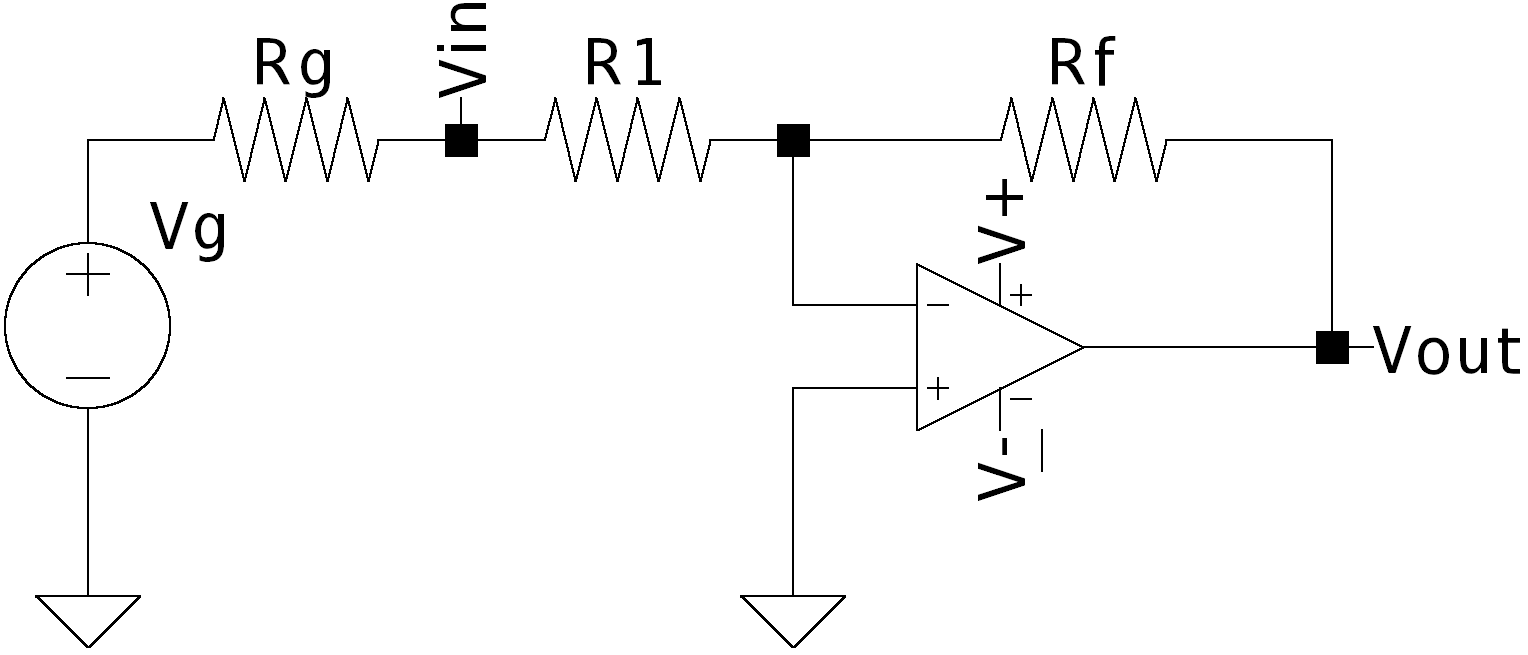
\includegraphics[width=0.5\textwidth]{images/circuit_inv}
\caption{\footnotesize Rappresentazione a costanti concentrate del circuito utilizzato.
  Si mettono in evidenza, oltre alle resistenze $R_{1}$ e $R_{\text f}$, la resistenza del
generatore $R_{G}$.}\label{fig:wrapfig}
\end{wrapfigure}
%------------------------------------
\noindent Successivamente viene assemblato sulla breadboard il circuito rappresentato in Figura \ref{fig:wrapfig}
e si preleva il segnale nei punti $V_{in}$ e $V_{out}$ utilizzando le sonde
$10X$ collegate ai canali A e B dell'oscilloscopio. I valori delle resistenze utilizzati sono stati
misurati direttamente con il multimetro e sono riportati nella Tabella \ref{tab:resist}.
Inoltre, il Picoscope viene configurato in modo da compensare l'attenuazione del segnale dovuta dalla sonda e si fa erogare al generatore di funzioni incorporato un segnale sinusoidale di $1\,\si{kHz}$, con ampiezza picco-picco inizialmente di $0.2\, \si{\volt}$, aumentata gradualmente fino a $4\,\si{\volt}$.

\noindent Risolvendo il circuito e assumendo ideale l'amplificatore operazionale, ci si aspetta che
il segnale in ingresso venga amplificato di un fattore $G = R_{\text f}/R_{1}$.
Inoltre, il segnale di output sarà invertito rispetto a quello di ingresso, in modo
da soddisfare la relazione $V_{\text{out}}=-G\, V_{\text{in}}$. Facendo riferimento ai valori riportati
in tabella \autoref{tab:resist} ci aspetta quindi un guadagno pari a

%-----------------------------------
\begin{align}\label{e:guadagno}
  G &= \frac{R_{\text f}}{R_{1}} = 8.38 \pm 0.06,
  &
  \sigma_{G} &= G \sqrt{ \left( \frac{\sigma_{R_f}}{R_{\text{f}}} \right)^{2}  +
			\left( \frac{ \sigma_{R_{1}}}{R_{1}} \right)^{2}}
\end{align}
% ---------------------------------

%------------------------------
\renewcommand{\arraystretch}{1.1}
\begin{table}
\centering
\setlength{\tabcolsep}{10pt}
\begin{tabular}{ |c|c|c|  }
\hline
\multicolumn{3}{|c|}{Misure dirette delle resistenze} \\
\hline
Resistenza      & Valore & F.S.\\
\hline
$R_{1}$ & $8.10 \pm 0.04\,\si{k\Omega}$ &$20\,\si{k\Omega}$ \\
$R_{\text{f}}$ & $67.9 \pm 0.3\,\si{k\Omega}$ &$200\,\si{k\Omega}$ \\
\hline
\end{tabular}
\caption{\footnotesize Si mostrano in tabella i valori e le incertezze delle resistenze usate in questa sezione, misurati con il multimetro Tenma. È stato riportato anche il fondo scala usato.}
\label{tab:resist}
\end{table}
%-------------------------------------

\subsection{Simulazione del Circuito}\label{s:sim}
Con l'obbiettivo di studiare il comportamento ideale del circuito rappresentato in Figura \ref{fig:wrapfig} in un range significativo
di segnali di ingresso, vengono effettuate delle simulzioni della risposta del
circuito ad
%------------------------------------
\begin{wrapfigure}{r}{0.5\textwidth}
\centering
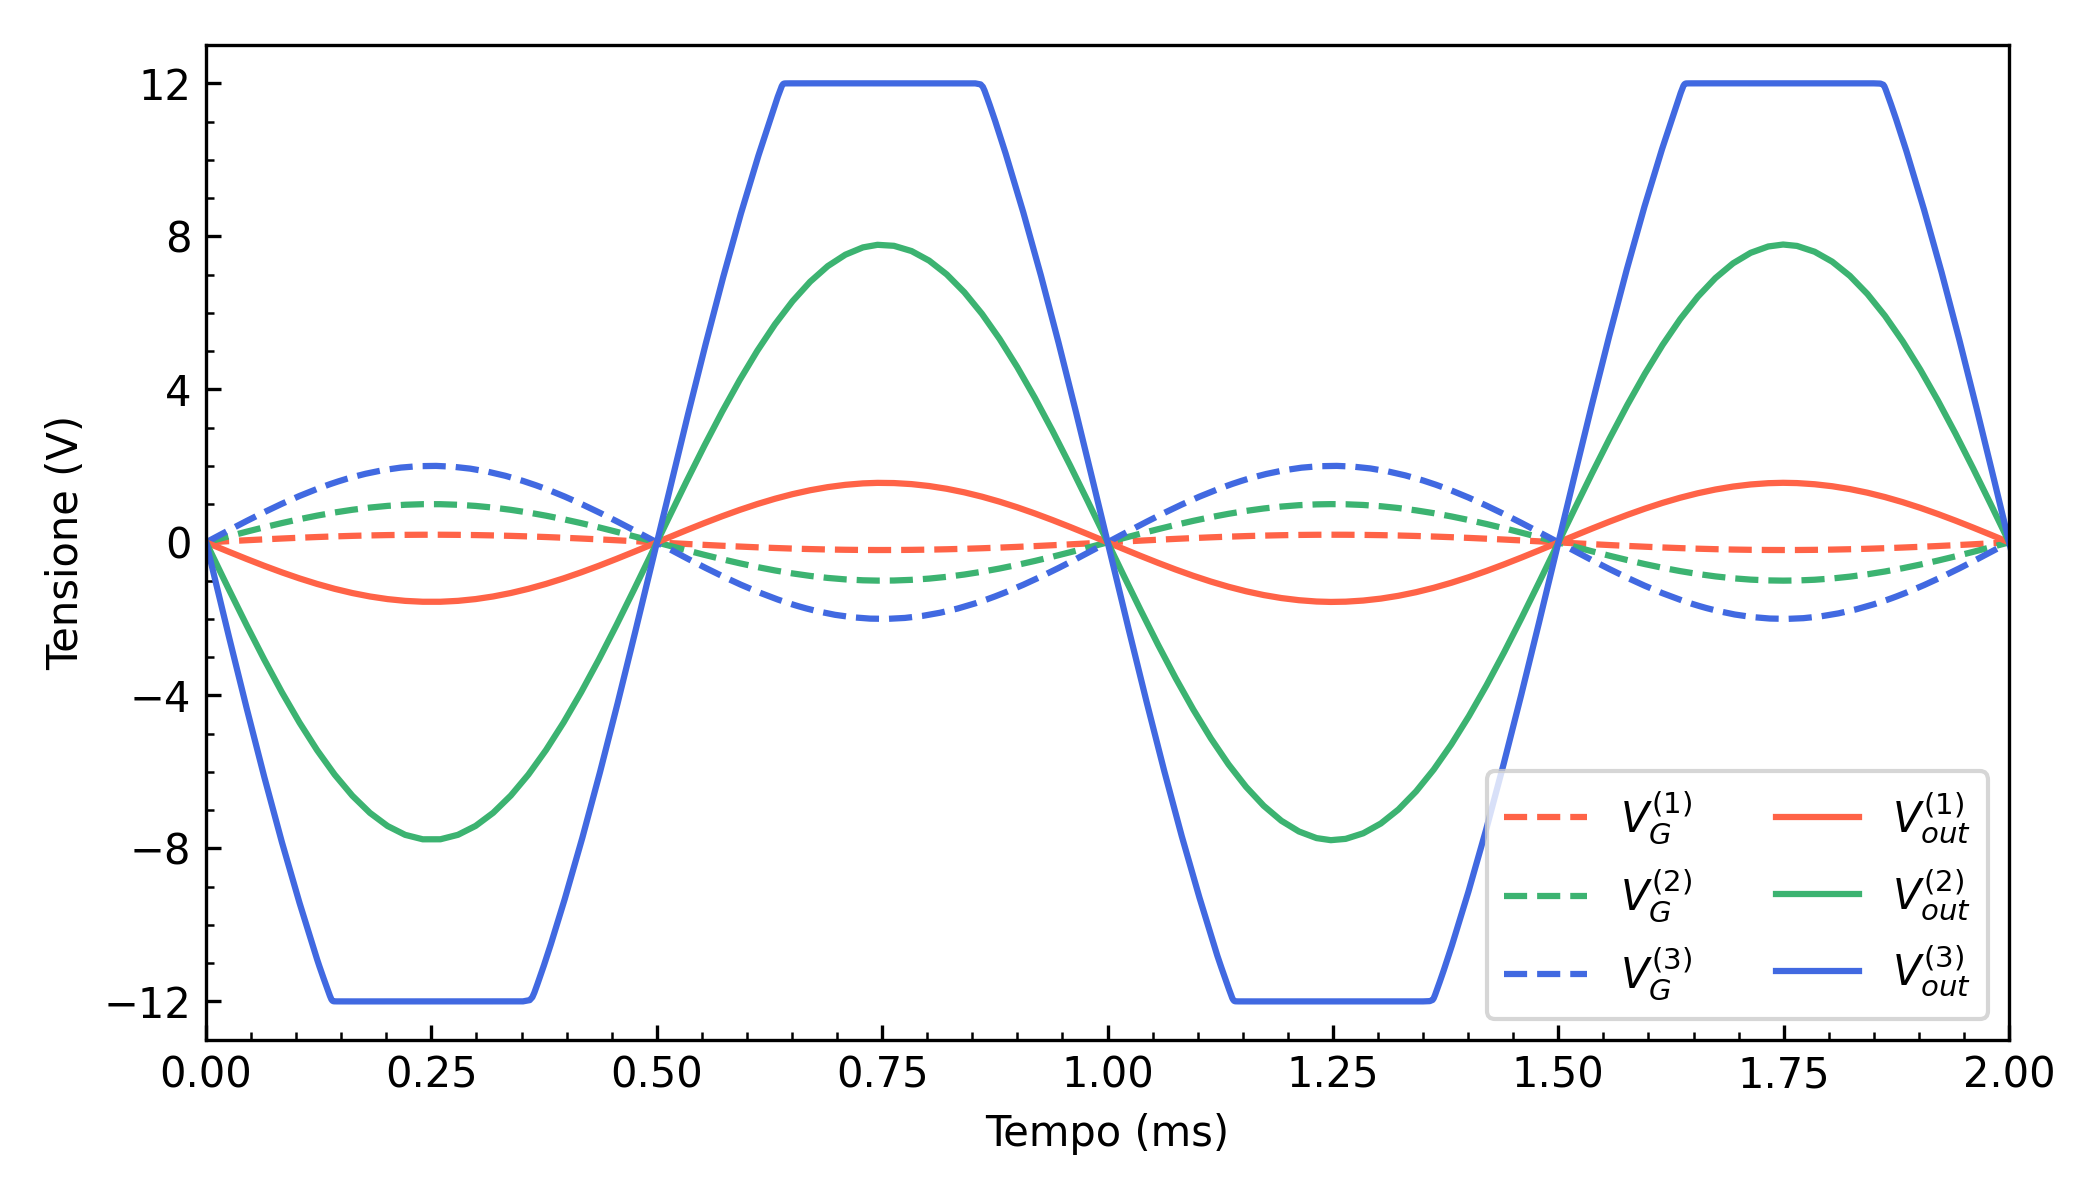
\includegraphics[width=0.5\textwidth]{images/lin_simulation}
\caption{\footnotesize Simulazione del circuito ottenuta con LTSpice XVII. Le linee
  tratteggiate rappresentano le tre tensioni di ingresso $V_{\text{gen}}^{(i)}$, mentre le linee continue rappresentano le corrispondenti tensioni di uscita $V_{\text{out}}^{(i)}$.}
\label{fig:lin_sim}
\end{wrapfigure}
%------------------------------------
un onda sinusoidale di $f_{\text{gen}}=1 \, \si{kHz}$, utilizzando il software LTspice
XVII. In particolare, sono state effettuate tre simulazioni, corrispondenti a tre ampiezze diverse
del segnale del generatore:
%-----------------------------------
\begin{align*} V_{G}^{(1)} &= 0.2 \, \si{\volt}
  &
	V_{G}^{(2)}&=1 \, \si{\volt}
  &
	V_{G}^{(3)}&=2 \, \si{\volt}
\end{align*}
%-----------------------------------
I risultati delle simulazioni sono riportati in Figura \ref{fig:lin_sim} e risulta evidente come le prime due simulazioni confermino le considerazioni svolte
nella sezione precedente: il segnale di uscita risulta infatti invertito rispetto al segnale di
ingresso, e amplificato di un fattore di circa $8$.
La terza simulazione, invece, evidenzia il fenomeno di saturazione dell'amplificatore operazionale: esso, infatti, è alimentato da
una tensione continua di $\pm 12 \,\si{\volt}$ e per conservazione dell'energia questa è
la tensione massima che può fornire in output. Come mostrato nel grafico quindi, i massimi e
minimi del segnale in usicta risultano tagliati alla tensione di saturazione.
Dato il guadagno trovato in Equazione \ref{e:guadagno}, ci si aspetta che questo fenomeno si verifichi già ad una tensione di input $V_{G}\, \approx 1.5\, \si{\volt}$.

\subsection{Procedura di Acquisizione Dati }
Sfruttando i cursori di tipo tensione dell'oscilloscopio, vengono registrati separatamente
i massimi e i minimi del segnale di ingresso $V_{1}$ e del segnale di uscita $V_{\text{out}}$,
aumentando progressivamente la tensione erogata dal generatore, partendo da un valore nominale
picco-picco di $V_{G}^{(pp)}=0.2 \, \si{\volt}$, fino a $V_{G}^{(pp)}=4 \, \si{\volt}$.
Data la resistenza non trascurabile del generatore $R_{G}\approx 600 \,\Omega$, occore
distinguere la tensione nominale del generatore $V_{G}$ e $V_{\text{in}}$, il valore letto
dall'oscilloscopio. Ci si aspetta che quest'ultimo sia minore, a causa del calo di tensione
dovuto dall resistenza interna del generatore.

\subsection{Analisi dei dati}
In questa sezione ci si propone innanzitutto di verificare l'accordanza dei dati sperimentali
con le misure acquisite. Successivamente si cerca di ottenere una stima migliore
dell'amplificazione del circuito $G$. Per fare ciò si riportano in grafico le coppie $V_{\text{in}}$ e
$V_{\text{out}}$ e tramite un'interpolazione lineare si tenta di ricavare la nuova stima di $G$.
Inoltre, studiando la bontà del fit, si cerca di valutare la validità dell'ipotesi di linearità.

\subsubsection{Selezione dei dati}
In Figura \ref{fig:lin_sim} vengono riportate le misure di $V_{\text{in}}$ e $V_{\text{out}}$, a cui è stata
associata l'incertezza di lettura sommata quadraticamente all'incertezza di scala
%----------------------------------
\begin{align}\label{e:err_misure}
  \sigma_{V_{i}}= \sqrt{ \left(\sigma_{r} \times \text{scala} \right)^{2} +
  \left( \sigma_{k} \times V_{i} \right)^{2}}
\end{align}
%----------------------------------
dove $\sigma_{k} = 1.7\%$ rappresenta l'errore di guadagno verticale dell'oscilloscopio. Come errore di lettura, si sceglie
di non utilizzare il valore fornito dal costruttore in quanto esso porterebbe ad
una sovrastima dell'errore. Si assume allora che il contributo maggiore all'errore di
lettura sia dato dalla discretizzazione che avviene durante la conversione analogico-digitale, per
cui l'errore massimo risulta $\Delta_{r}= 1 / 2^{n}$, dove $n$ rappresenta la risoluzione
dell'oscilloscopio. L'acquisizione delle misure è stata effettuata con $n=8 \text{ bit}$,
quindi, assumendo una distribuzione uniforme, si ha $\sigma_{r} = 0.002$.
Infine, nel caso del Picoscope, la scala rappresenta l'ampizza dell'intervallo impostato come range
sull'oscilloscopio.
%------------------------------------
\begin{figure}[h]
\centering
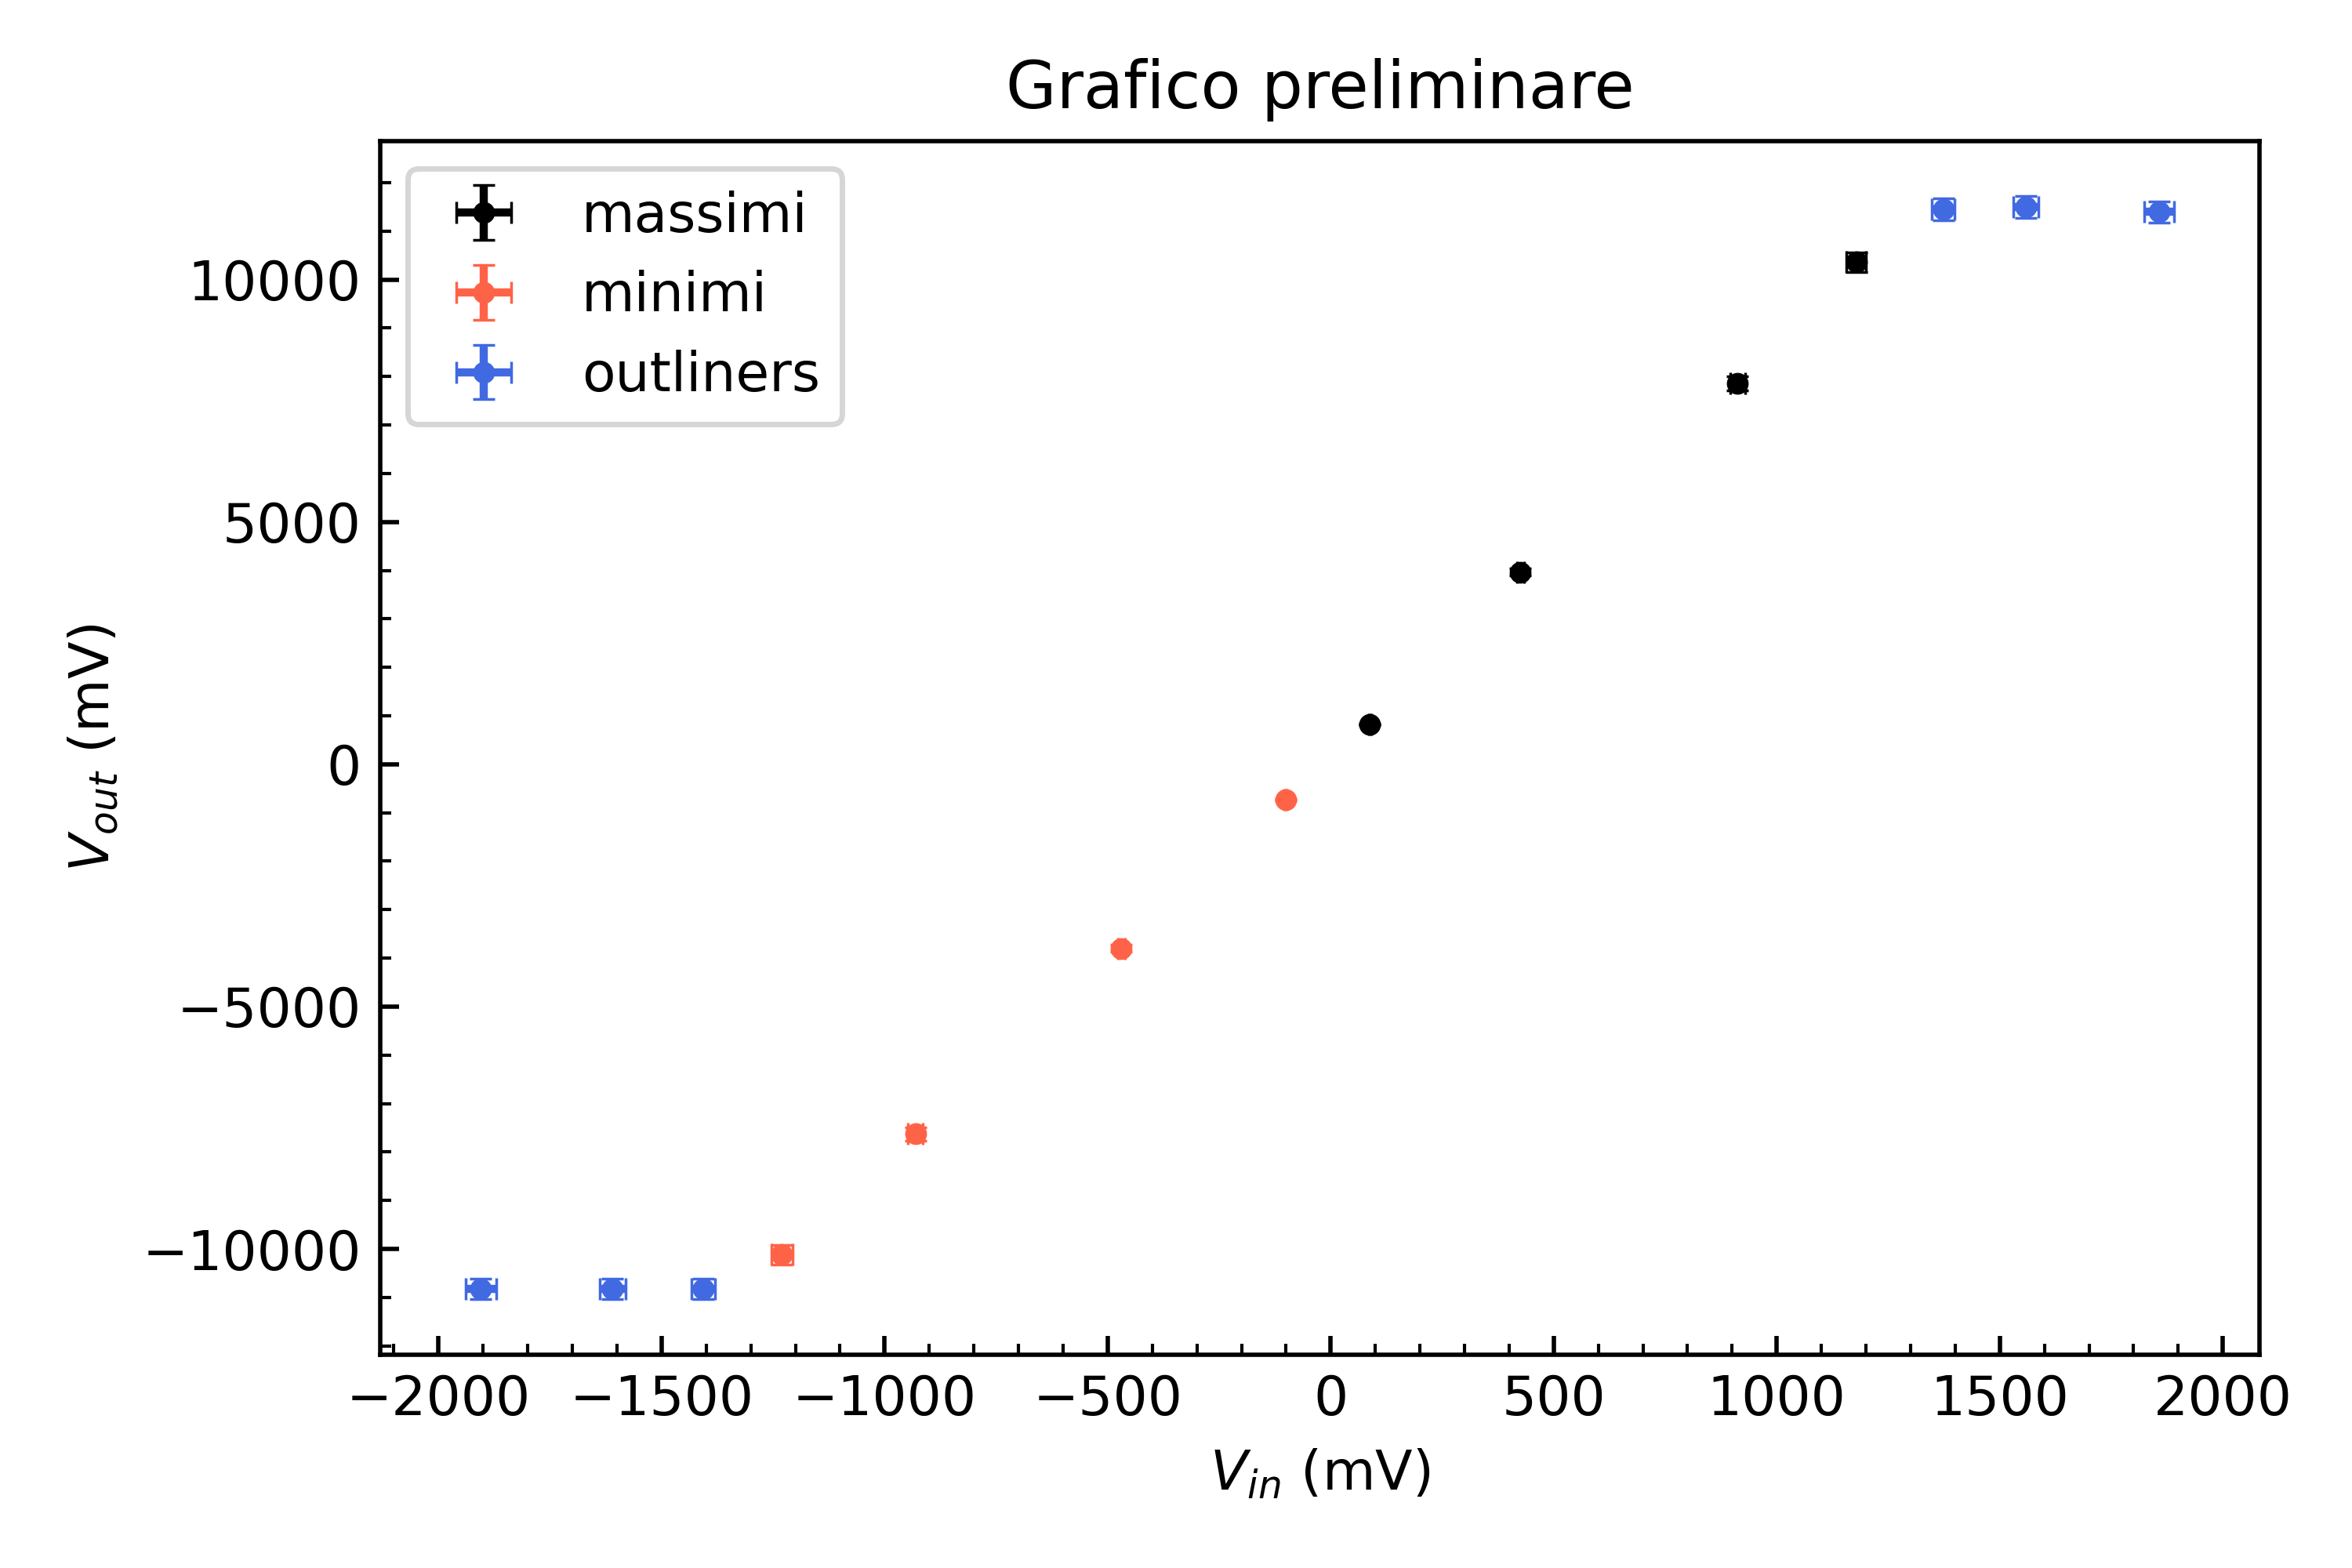
\includegraphics[width=0.7\textwidth]{images/grafico_esplorativo}
\caption{\footnotesize Grafico preliminare delle coppie $(V_{in},V_{out})$ dei massimi (in nero) e dei minimi (in rosso). Gli outliners dovuti al fenomeno di saturazione sono
evidenziati in blu.}\label{fig:lin_prelim}
\end{figure}
%------------------------------------

Dalla Figura~\ref{fig:lin_prelim} si può subito osservare come i valori di $V_{\text{out}}$ siano amplificati di un
fattore di circa $8$, coerente con le aspettave. Inoltre, i valori della tensione in ingresso sono affetti dalla
caduta di potenziale rispetto al valore nominale della tensine del generatore, come previsto. Si nota infine
il fenomeno di saturazione descritto nella Sezione \ref{s:sim}. Gli outliners corrispondenti non verranno
considerati nelle analisi successive.

\subsubsection{Interpolazione Lineare}\label{s:lin_fit}
Si procede ora con la suddivisione dei dati in due set, corrispondenti ai massimi e ai minimi,
con l'obbiettivo di effettuare un interpolazione lineare su ciascun campione e, dopo aver verificato
la compatibilità tra i parametri dei fit, fare una nuova interpolazione sui set unificati.
Non è infatti possibile stabilire a priori se l'amplificazione sia la stessa tra i due set
e se ci siano eventuali sfasamenti tra i due fit. Il coefficiente angolare dell'interpolazione
rappresenta una nuova stima dell'amplificazione $G$ e ci si aspetta che l'intercetta risulti
compatibile con lo zero.
Si noti però che gli errori associati alle ascisse ($V_{\text{in}}$) non risultano trascurabili rispetto a
quelli associati alle ordinate ($V_{\text{out}}$). Si decide allora di eseguire un primo fit senza considerare
l'errore sulle ascisse, per poi utilizzare il coefficiente angolare di questa interpolazione per proiettare gli errori
di $V_{\text{in}}$ sulle ordinate, secondo la formula
%--------------------------------------
\begin{align}\label{e:proiezione}
 \sigma_{y} = \sqrt{ (m \times \sigma_{V_{in}})^{2} + \sigma_{V_{out}}^{2}}
\end{align}
%--------------------------------------
I risultati dei quattro fit sono riportati nella Tabella \ref{tab:fitmaxmin}. Si osservi però che il limitato numero
di misure di ciascun campione rende i fit poco significiativi e si attribuisce proprio a
questo problema la discrepanza tra gli errori a posteriori del fit dei massimi e quello dei
minimi: i primi infatti indicherebbero una leggera sottostima degli errori mentre i secondi
suggeriscono una forte sovrastima, che si rispecchia anche in un $\chi^{2}$ eccessivamente ridotto. I coefficienti angolari delle rette risultano inoltre scarsamente compatibili tra di loro ($\lambda = 2.2$). La compatibilità tra le due intercette risulta tuttavia ottima ($\lambda = 0.97$), ma la loro compatibilità con lo zero è discreta nel caso dei massimi ($\lambda = 1.83$), mentre nel caso dei minimi l'intercetta risulta addirittura incompatible
con lo zero ($\lambda = 3.21$).
\begin{table}[h]
\centering
\setlength{\tabcolsep}{10pt}
\begin{tabular}{ | c c | c c | c c | c c|  }
\hline
  \multicolumn{8}{|c|}{Parametri dei fit} \\
  \hline
  \multicolumn{4}{|c|}{Massimi} &
  \multicolumn{4}{c|}{Minimi} \\
  \hline
  \multicolumn{2}{|c}{$m_{\text{pre}}$} & \multicolumn{2}{c|}{$8.80 \pm 0.11$} &
  \multicolumn{2}{c}{$m_{\text{pre}}$} & \multicolumn{2}{c|}{$8.32 \pm 0.10$} \\
  $m_{\text{max}}$   &   $8.80 \pm 0.16$             &   $\sigma_{\text{p}}$              &   $ 202 \,\si{m\volt}$   &   $m_{\text{min}}$   & $8.32 \pm 0.15 $            &  $\sigma_{\text p}$             & $10 \,\si{m\volt}$ \\
  $q_{\text{max}}$   &   $ 64 \pm 35 \,\si{m\volt}$   &   $\chi^{2}/\text{ndf}$           &   $3.9/2$   &   $q_{\text{min}}$   & $110 \pm 35 \, \si{m\volt}$  & $\chi^{2} / \text{ndf}$        & $0.01/2$ \\
\hline
\end{tabular}
\caption{\footnotesize Si mostrano in tabella i coefficienti angolari dei fit preliminari
  $m_{\text{pre}}$ e i risultati dei fit con gli errori proiettati: in particolare si mostrano i
  coefficienti angolari $m_{i}$, le intercette $q_{i}$, gli errori a posteriori
  $\sigma_{\text{p}}$ e il chi quadro $\chi^{2}$ in relazione ai suoi gradi di libertà.}
\label{tab:fitmaxmin}
\end{table}

\noindent Si noti infine che nell'interpolazione sono stati considerati
sia i contributi degli errori di lettura che quelli di di guadagno verticale, in quanto
l'acquisizione delle misure è avvenuta a scale diverse. Questo tuttavia introduce una
correlazione tra le misure di cui il fit lineare non tiene conto e che quindi porta ad una
sottostima degli errori sui parametri e ad una compatibilità peggiore tra i due set.
Tuttavia, nonostante queste considerazioni, l'incompatibilità dell'intercetta dei minimi con
lo zero non può essere ignorata: essa infatti suggerisce un possibile errore sistematico di offset e vista la ottima compatibilità con l'intercetta del fit dei massimi si può assumere che
tale sistematica sia presente in entrambi i set e che sia costante, ovvero che si tratti di
una interferenza di fondo. Sebbene uno shift verticale costante non influenzi il coefficiente angolare dell'interpolazione (cioè la nuova stima di $G$) si sceglie comunque di non
unire i due campioni, ma di analizzare le grandezze picco-picco delle tensioni in ingresso e in uscita,
secondo la formula $V_{\text{pp}}=V_{\text{max}} - V_{\text{min}}$. In questo modo infatti, non solo si dovrebbe
riuscire a eliminare il contributo di errore di shift verticale comune a
entrambi i set, ma è possibile ridurre anche un eventuale sistematicha di offset tra i due campioni, purchè
costante per tutti i dati.\\

\noindent Come mostrato in precedenza, si procede prima con un fit
preliminare in cui si trascura il contributo degli errori delle ascisse, per poi
sfruttare il coefficente angolare così ottenuto per proiettare gli errori sulle ordinate secondo l'Equazione \ref{e:proiezione}, potendo così fare un nuovo fit che tiene conto di
entrambe le incertezze. Nella Figura \ref{fig:lin_pp} sono riportati i risultati del fit.
%------------------------------------
\begin{figure}[h]
\centering
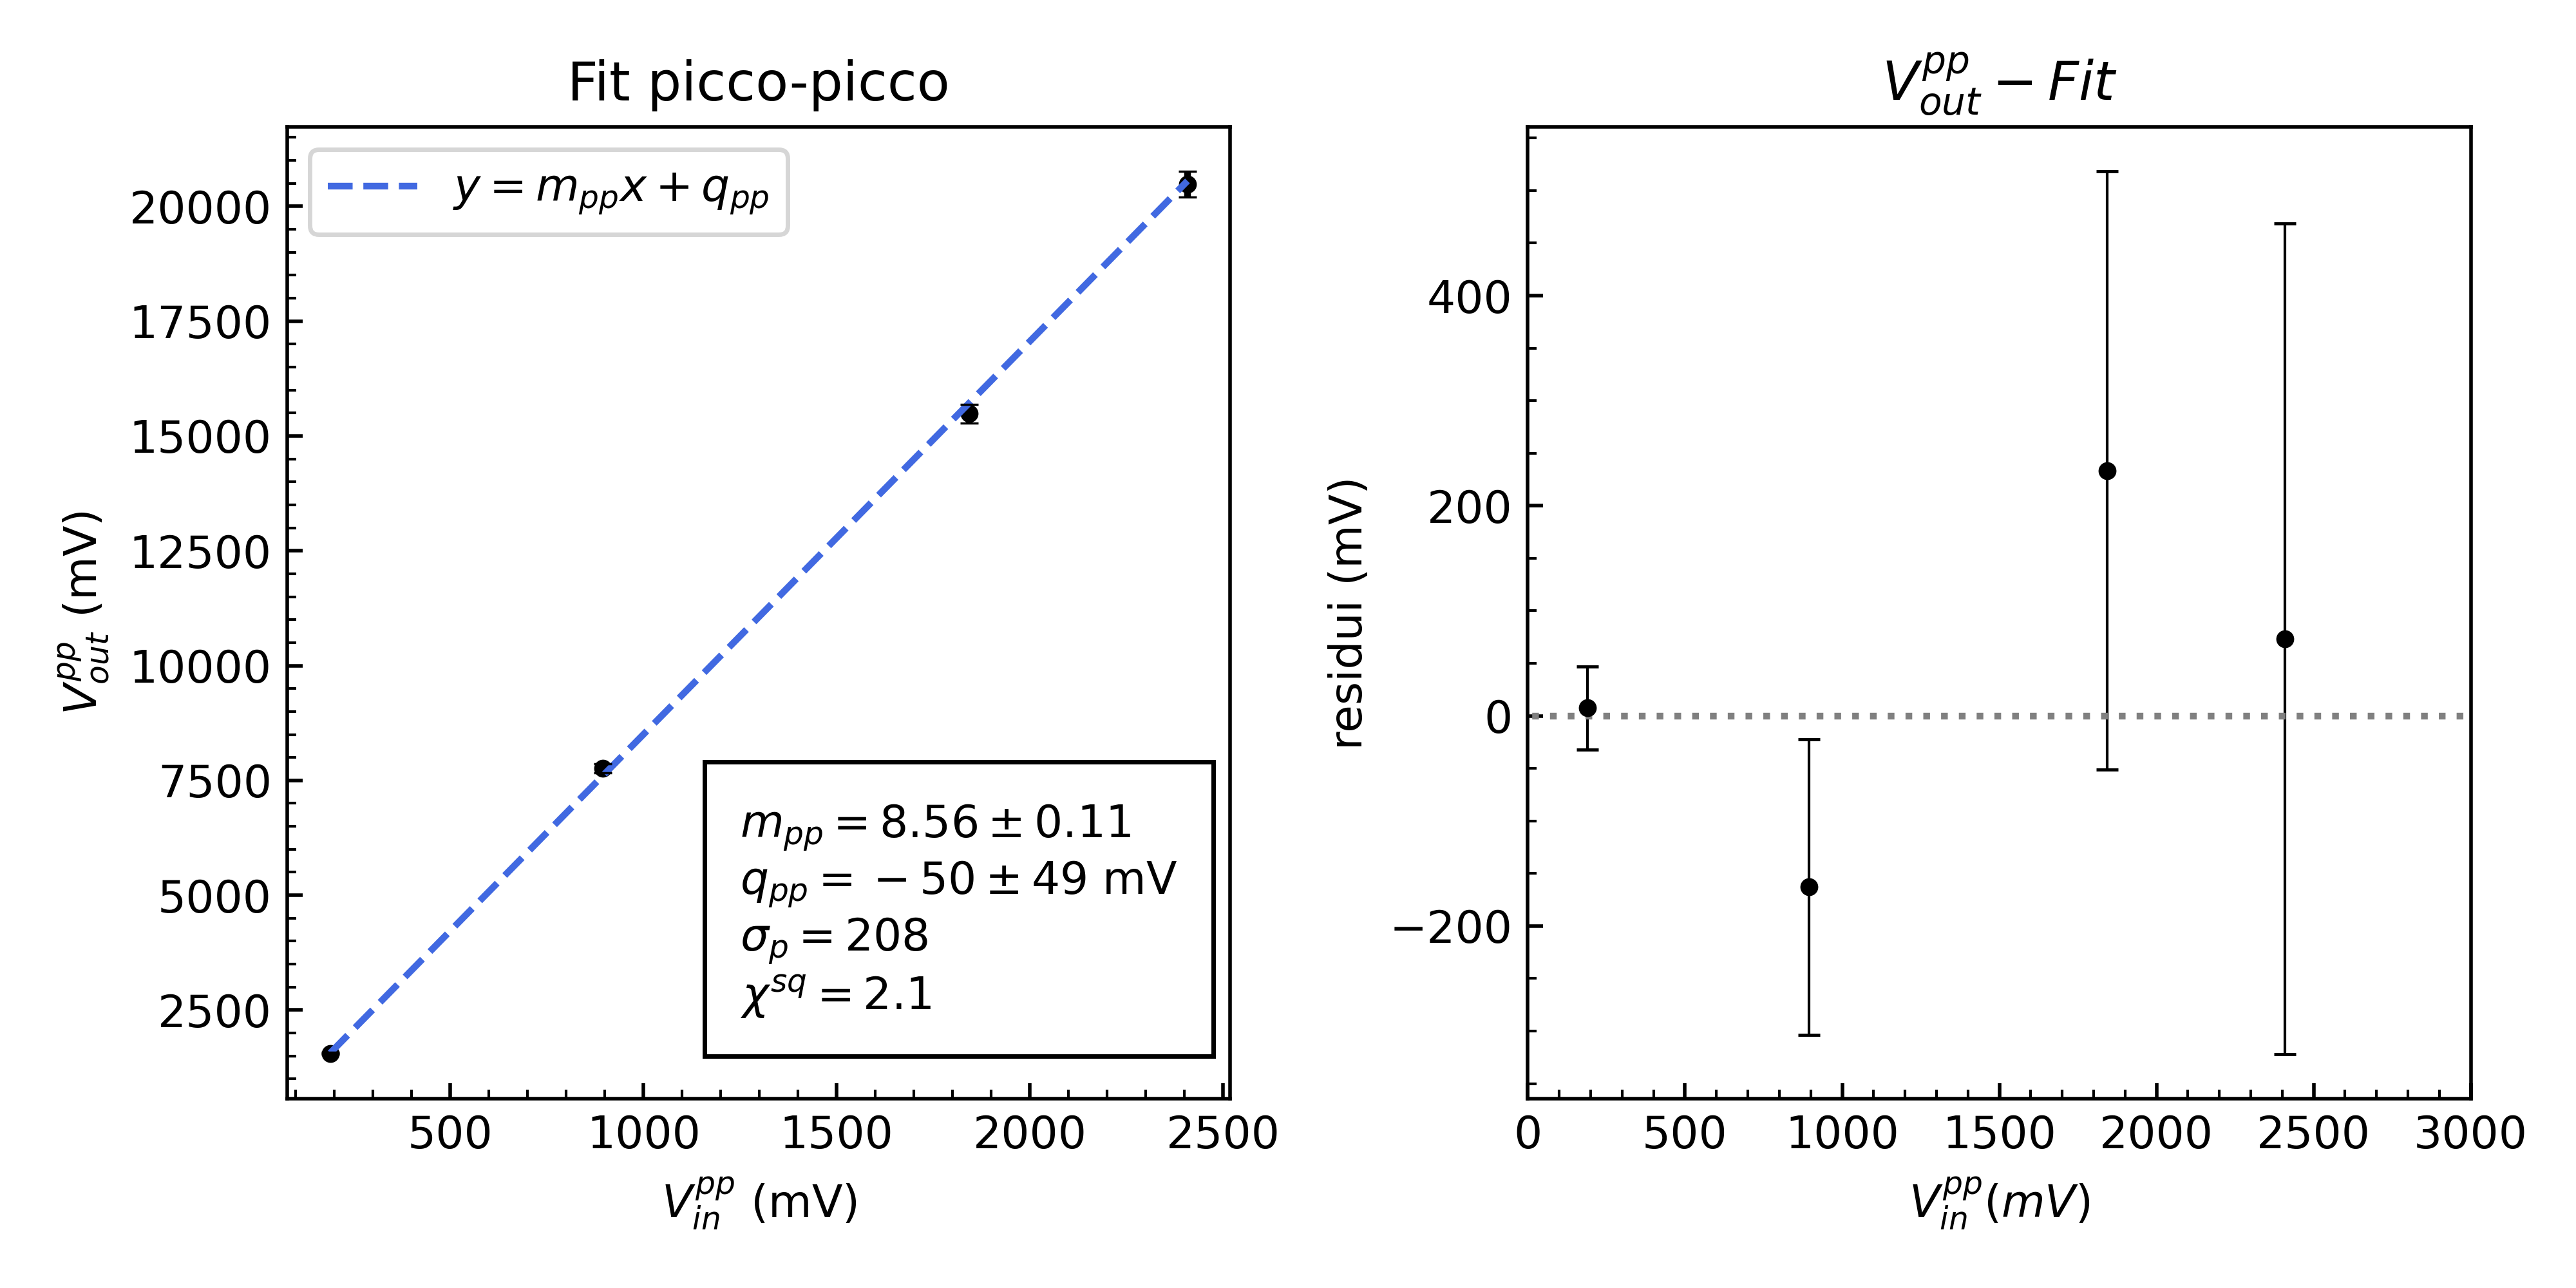
\includegraphics[width=0.9\textwidth]{images/grafico_pp}
\caption{\footnotesize Si mostra in figura il grafico dell'interpolazione dei dati picco-picco coi relativi
residui. Vengono inoltre riportati i parametri più significativi del fit.}\label{fig:lin_pp}
\end{figure}
%------------------------------------
Si noti come la compatibilità dell'intercetta con lo zero sia ora $\lambda=1.0$, confermando quindi l'ipotesi di un offset verticale comune a entrambi i set e che è stato rimosso una volta
presa la differenza. Anche il chi quadro risulta ora perfettamente compatibile con i suoi
gradi libertà ($\lambda=1.0$), confermando quindi l'ipotesi di andamento lineare dei
dati. Il coefficiente angolare, che rappresenta la nostra stima dell'amplificazione $G$,
risulta discretamente compatibile con il valore teorico previsto dall'Equazione
\ref{e:guadagno} ($\lambda = 1.4$).
Dal grafico dei residui si evidenzia inoltre una buona stima degli errori, con l'eccezione
dell'ultimo dato in cui l'incertezza è stata chiaramente sovrastimata.
Data la forte presenza di errori sistematici, si è scelto di non proseguire con l'analisi di
ulteriori indicatori indicatori statistici.

\subsubsection{Stime di G}
In Figura \ref{fig:all} sono state riportate tutte le stime dell'amplificazione $G$ del circuito calcolate nei paragrafi precedenti: dai coefficienti angolari dei fit dei massimi e dei
minimi sono state ottenute due stime $G_{\text{max}}$, $G_{\text{min}}$, compatibili tra di loro
($\lambda_{\text{max/min}}=2.2$), anche se debolmente. Da queste due stime si dicide di effettuare una media pesata, anchessa riportata in Figura \ref{fig:all}, ottenendo così un nuovo valore $<G>$ in ottimo accordo con la stima $G_{\text{pp}}$ ottenuta dall'analisi picco picco ($\lambda_{\text{pp/<>}}=0.1$). Queste ultime due stime presentano
inoltre una buona compatibilità con il valore $G_{\text{th}}$ previsto dall'Equazione \ref{e:guadagno}
$(\lambda_{\text{<>/th}} \approx \lambda_{\text{pp/th}} = 1.4)$.
Nonstante però tali compatibilità siano inferiori rispetto all'accordo che ha $G_{\text{min}}$ con l'aspettativa teorica ($\lambda_{\text{min/th}}=1.11$), si decide comunque di assumere come stima migliore dell'amplificazione
del circuito $G_{\text{pp}}$ in quanto si tratta del valore meno influenzato da errori sistematici, come spiegato nella Sezione \ref{s:lin_fit}.
%------------------------------------
\begin{figure}[h]
\centering
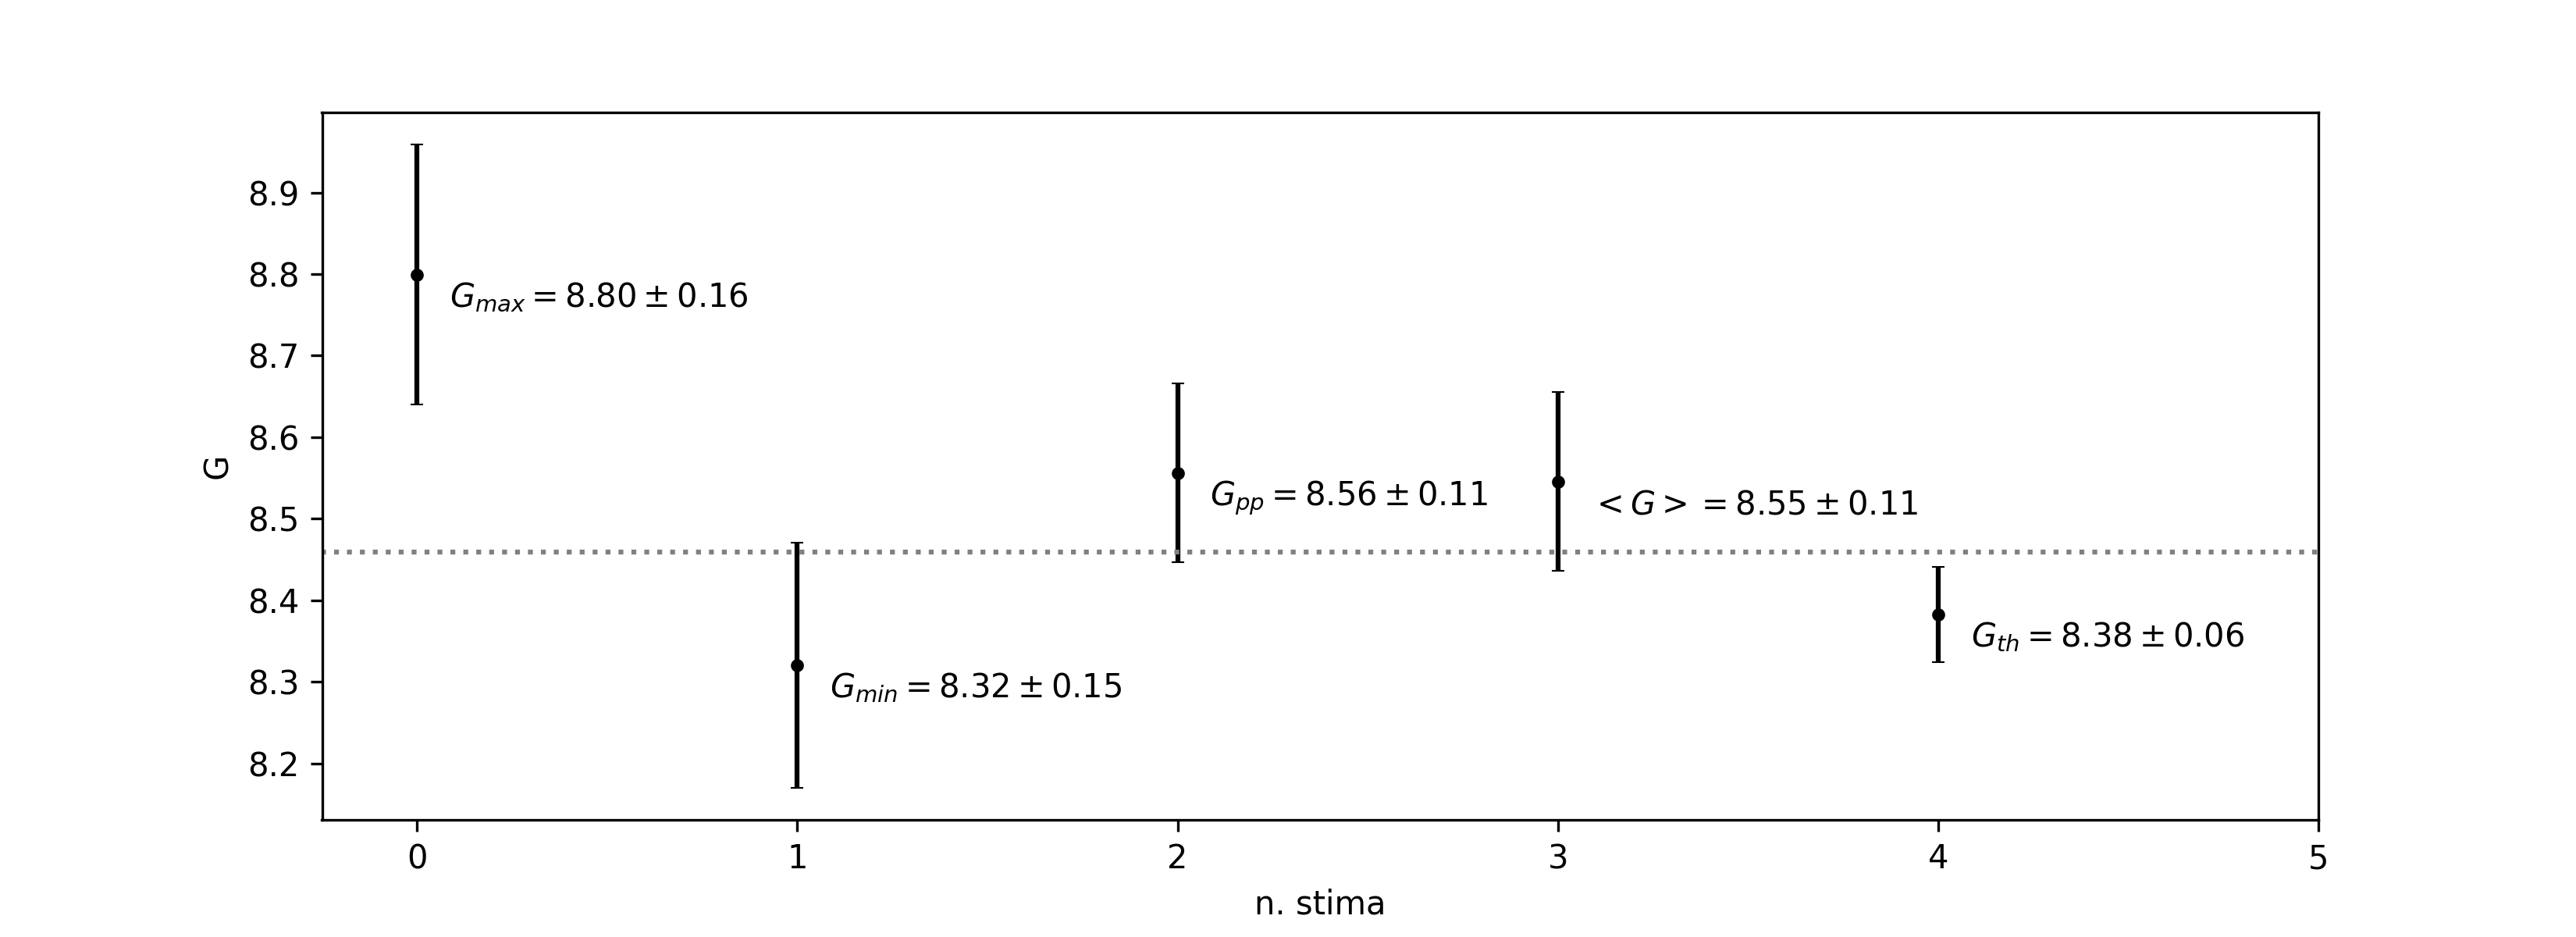
\includegraphics[width=0.9\textwidth]{images/grafico_all}
\caption{\footnotesize Nel grafico vengono presentate tutte le stime dell'amplificazione del circuito.
  In ordine da sinistra verso destra: 0) stima ottenuta partendo dal set di massimi, 1) dal set di minimi,
  2) dai valori picco-picco 3) dalla media pesata dei massimi e minimi, 5) aspettativa teorica.
}\label{fig:all}
\end{figure}
%-------------------------------------

\section{Circuito Derivatore}
\label{sec:circuito-derivatore}

In questa sezione ci si propone di studiare la risposta in frequenza del circuito
rappresentato in Figura~\ref{fig:circ_bode}. Si tratta di un filtro attivo passa alto e derivatore a basse
frequenze. In particolare, si vuole stimare la frequenza di taglio e confrontarla con le
aspettative teoriche e con le simulazioni.
%-------------------------------------
\begin{figure}[h]
\centering
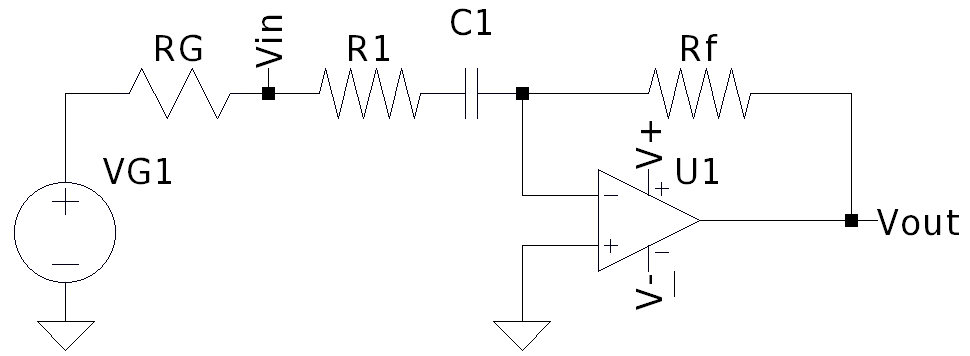
\includegraphics[width=0.5\textwidth]{images/circuit_bode}
\caption{\footnotesize Rappresentazione a costanti concentrate del ciruito
  derivatore utilizzato. Si mette in evidenza la resistenza non trascurabile del generatore $R_G$ che implica una tensione $V_{\text{in}}$ inferiore rispetto a quella nominale del generatore di funzioni.}\label{fig:circ_bode}
\end{figure}
%-------------------------------------

\subsection{Configurazione Sperimentale}\label{sec:confspeDeriv}

Il circuito viene realizzato aggiungendo a quello mostato in Figura~\ref{fig:wrapfig} la
capacità $C_1= 2.05\pm 0.05 \,\si{n\farad}$. In questo modo ci si aspetta che la frequenza di taglio sia
\begin{align}
  \label{eq:f_teo}
  f_{\textrm t} &= \frac{1}{2\pi R_1 C_1} = 9.6 \pm 0.2 \, \si{k\Hz}
  &
  \sigma_{f_{\textrm t}} &= f_t \sqrt{ {\left( \frac{\sigma_{R_1}}{R_1} \right)}^2+
  \left( \frac{\sigma_{C_1}}{C_{1}} \right)^{2}} 
\end{align}
Si è quindi configurato il generatore di
funzioni in modo tale da erogare un'onda triangolare di ampiezza $1 \V$ e frequenza $1 \,\si{k\Hz}$, con
l'obbiettivo di verificare il funzionamento da derivatore. Successivamente si ripristina la
forma d'onda sinusoidale per ricavare una primia stima sperimentalmente della frequenza di taglio,
modificando opportunamente la frequenza del generatore e osservando l'amplificazione ottenuta. Ci si aspetta
infatti che in corrispondenza della frequenza di taglio valga la relazione
\begin{align}
  \label{eq:h_teo}
  H(f_{\text t}) &= \frac{1}{\sqrt 2} \frac{R_{\textrm f}}{R_{1}} =  \frac{G}{\sqrt 2} =  5.93 \pm 0.04
  &
  \sigma_{H_{\textrm f}} & = \frac{\sigma_{G}}{\sqrt 2}
\end{align}
dove $H=|Vout/Vin|$ rappresenta la funzione di trasferimento, mentre $G$ è il guadagno calcolato
in Equazione \ref{e:guadagno}.\\
Infine, per studiare la risposta in frequenza del circuito e ottenere una stima più precisa
della frequenza di taglio, si decide di variare
la frequenza del generatore tra $10 \,\si{k\Hz}$ e $100 \,\si{k\Hz}$
e di registrare l'amplificazione del segnale. Si prevede che la funzione di trasferimento sia data da
\begin{align}
  \label{eq:1}
  H(\omega) &= \frac{\omega}{\sqrt{\omega^{2} + \omega_{0}^{2}}}
              \frac{R_{\textrm f}}{R_{1}}
  &
  \omega_{0} & = \frac{1}{R_{1} C_{1}}
\end{align}
Ci si aspetta quindi che il circuito si comporti come un derivatore a basse frequenze e che si ottenga il guadagno massimo $G$ per $\omega \to \infty$.

\subsection{Procedura di Acquisizione Dati}
\label{sec:acqu-delle-misure}
Innanzitutto, si registra la risposta del circuito ad un'onda triangolare
di ampiezza $1 \V$ e frequenza $1 \, \si{k\Hz}$. Si riporta in Figura \ref{fig:screen_deriv}
uno screenshot dell'output dell'oscilloscopio. Si osserva che la risposta è
un'onda quadra, ovvero la derivata del segnale di ingresso. Si conferma
quindi l'ipotesi di circuito derivatore. Si riscontrano tuttavia delle
deformazioni nell'onda quadra, attribuibili all'alta frequenza dell'onda di
ingresso: trattandosi di un filtro passa alto infatti, ci si aspetta che
il comportamento da derivatore sia più accentuato a basse frequenze.

%------------------------------------
\begin{wrapfigure}{r}{0.5\textwidth}
\centering
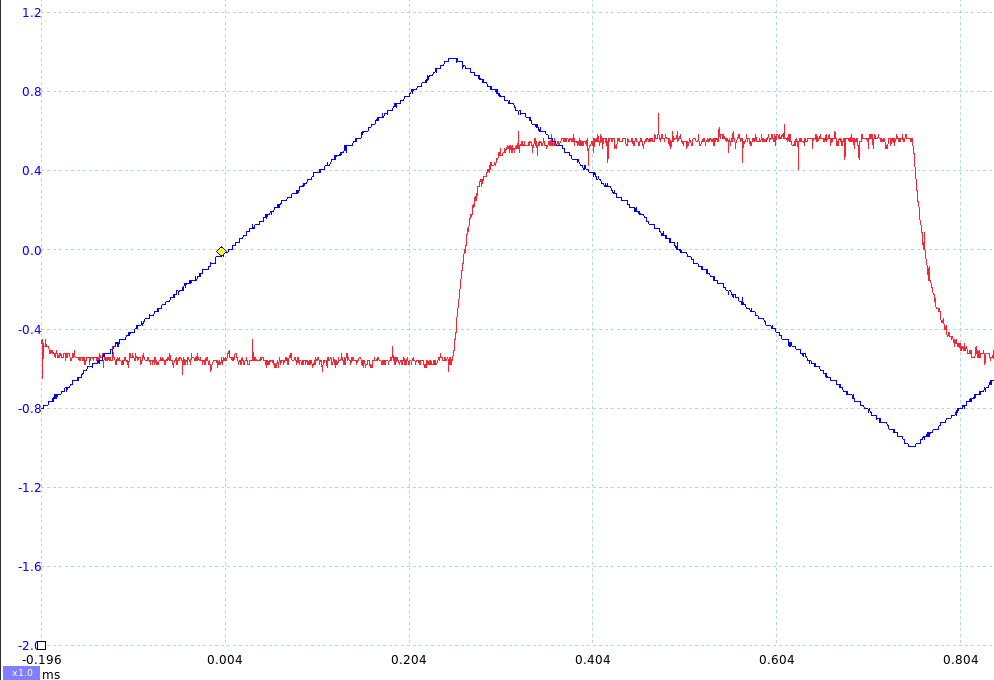
\includegraphics[width=0.5\textwidth]{images/screen_deriv}
\caption{\footnotesize Screenshot dell'oscilloscopio con un'onda triangolare in input.
Si osserva in output un'onda quadra deformata.}
\label{fig:screen_deriv}
\end{wrapfigure}
%------------------------------------

\noindent Successivamente, come anticipato, si
configura in ingresso un'onda sinusoidale di ampiezza $1 \V$
e si registrano i valori $V_{\textrm{in}}$ e $V_{\textrm{out}}$, modificando la
frequenza del generatore di funzioni fino ad ottenere un'amplificazione compatible con quella calcolato nell'Equazione \ref{eq:h_teo}.  Si stima così una frequenza di taglio di $f_{t} \approx 9.5 \,\si{k\Hz}$.\\
Si procede poi
con un'analisi più dettagliata del comportamento in frequenza, variando
la frequenza del generatore da $100 \,\si{\Hz}$ a $100 \,\si{k\Hz}$ e campionando un numero maggiore di ampiezze $V_{\text{in}}$ e $V_{\text{out}}$
in prossimità della frequenza di taglio appena calcolata.
Si osserva subito un primo discostamento dall'aspettativa teorica: si registra in fatti un'attenuazione del guadagno per frequenze elevate, in chiara contraddizione con le
considerazioni della Sezione \ref{sec:confspeDeriv}, in cui si era previsto un aumento dell'amplificazione per valori di frequenza maggiori.

\subsection{Dati e analisi}
Si vuole ora riassumere la risposta in frequenza del circuito tramite un grafico di Bode e confrontarlo cone le simulazioni di LTspice. Si procede poi
con la stima della frequenza di taglio in due metodi alternativi: in un primo
momento tramite delle interpolazioni lineari e paraboliche del grafico di bode,
e in seguito da un fit in scala lineare di un intorno della frequenza di taglio.

\subsubsection{Grafico di Bode}
\label{sec:grafico-di-bode}

Per realizzare il grafico di Bode a partire dalle coppie $(V_{\text{in},i}, V_{\text{out},i})$ si
calcola il lograritmo della funzione di trasferimento
\begin{align}
  \label{eq:3}
  H_{i} &=\frac{V_{\text{out},i}}{V_{\text{in},i}}
  &
    \sigma_{H,i} &= H_{i}\sqrt{ \left(\frac{\sigma_{\text L} \times \text{scala}_{\text{in},i}}{V_{\text{in},i}} \right)^{2} +
                 \left( \frac{\sigma_{\text L} \times \text{scala}_{\text{out},i}}{V_{\text{out},i}} \right)^{2}}
\end{align}
%TODO: sostituisci V/div con scala
dove $\sigma_{L}=0.002$ rappresenta l'errore di lettura dell'oscilloscopio mentre $scala_{\text{in},i}$ e $scala_{\text{out},i}$ sono le
scale utilizzate per l'acquisizione del segnale in ingresso e in uscita rispettivamente. L'errore di scala
non viene invece considerato in quanto, prendendo il logaritmo, il guadagno si trasferisce sull'intercetta.

%------------------------------------
\begin{wrapfigure}{r}{0.5\textwidth}
\centering
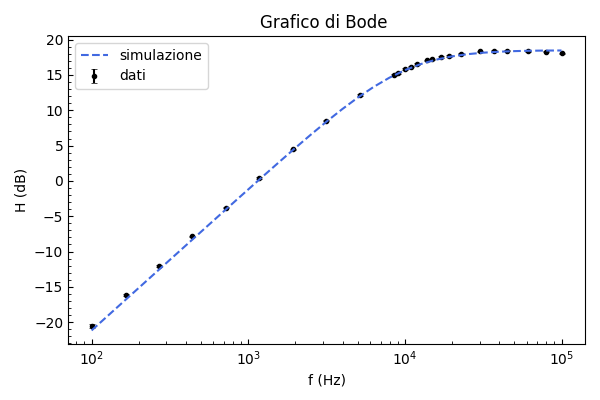
\includegraphics[width=0.5\textwidth]{images/grafico_bodeSim}
\caption{\footnotesize Grafico di Bode dei dati sperimentali confrontato con la simulazione LTspice.}
\label{fig:graf_bode}
 \vspace{-10pt} % This removes the white box on the second page
\end{wrapfigure}
%------------------------------------

\noindent In Figura \ref{fig:graf_bode} è rappresentato il grafico di Bode, in cui le funzioni di trasferimento sono riportate in decibel e
le ascisse vengono rappresentate in scala logaritmica. Nel grafico viene riportata anche la simulazione LTspice, che
evidenzia un ragionevole accordo con i dati sperimentali. Tuttavia, a frequenze elevate si nota il fenomeno di attenuazione del guadagno osservato nella sezione \ref{sec:acqu-delle-misure}. Si prevede che per frequenze superiori questa anomalia
risulti ancora più evidente. Ci si ritiene comunque soddisfatti dell'andamento dei dati rispetto alla simulazione, soprattuto considerando l'ampio range di frequenze  che si sta analizzando.
Si cerca ora di stimare la frequenza di taglio e, osservando che i punti del grafico di Bode seguono sostanzialmente due andamenti, si decide di effettuare due fit: uno parabolico ($y=a x^{2}+b x + c$) e uno lineare ($y=d x+ e$). I risultati di entrambi sono riportati in Figura \ref{fig:fit_bode}.
Dalla prima interpolazione si stima il massimo $H_{\text{max}}$ della funzione di trasferimento dal vertice della parabola

\begin{align}
  \label{eq:4}
  x_v &= - \frac{b}{2a} & H_{\text{max}}&=-\frac{b^2}{4a}+c=18.45 \pm 0.04 \, \si{dB}
   \end{align}
dove l'errore su $H_\text{max}$ viene calcolato con la formula
\begin{equation}
\sigma_{H_{max}}  =\sqrt{x_v\left[x_v^3\sigma_a^2 + 2x_v^2\text{cov}(a,b)+  x_v(\sigma_b^2+2\text{cov}(a,c))+2\text{cov}(b,c)\right]+\sigma_c^2} 
\end{equation}
Dal fit lineare invece si ricava l'ascissa per cui la retta vale $H_{max}$, tale $x$ rappresenta la stima della frequenza di taglio
\begin{gather}
  \label{eq:5}
  f_{t} = \frac{H_{\text{max}} - e}{d}=4.009\pm0.006 \, \text{dec}\\ 
  \sigma_{f_{t}} = f_t\sqrt{  \left( \frac{\sigma_{H_{\text{max}}}}{H_{\text{max}}-e}\right)^2 + 
	  \left( \frac{\sigma_d}{d}\right)^2 + 
	  \left( \frac{\sigma_e}{H_{\text{max}}-e}\right)^2 + 
  2 \frac{\text{cov}(e,d)}{(H_\text{max}-e)d}}
\end{gather}
Si converte infine il risultato ottenuto in $\si{\Hz}$, ottenendo 
$f_{t}=10.21\pm0.14 \,\si{k\Hz}$.
La frequenza di taglio così ottenuta risulta debolmente compatibile con
quella stimata con l'Equazione \ref{eq:f_teo} ($\lambda=2.5$). Dal grafico dei residui si osserva però una componente sistematica
particolarmente evidente nella regione lineare, in cui i residui seguono un chiaro andamento
parabolico. Si crede che questo comporti una stottostima del coefficiente angolare $d=19.31 \pm 0.10$ dB/dec, incompatibile con l'aspettativa teorica $d_{th}=20$ dB/dec, e che si traduce in una sovrastima della frequenza di taglio, giustificando quindi la scarsa compatibilità con l'aspettativa teorica.
%-------------------------------------
\begin{figure}[h]
\centering
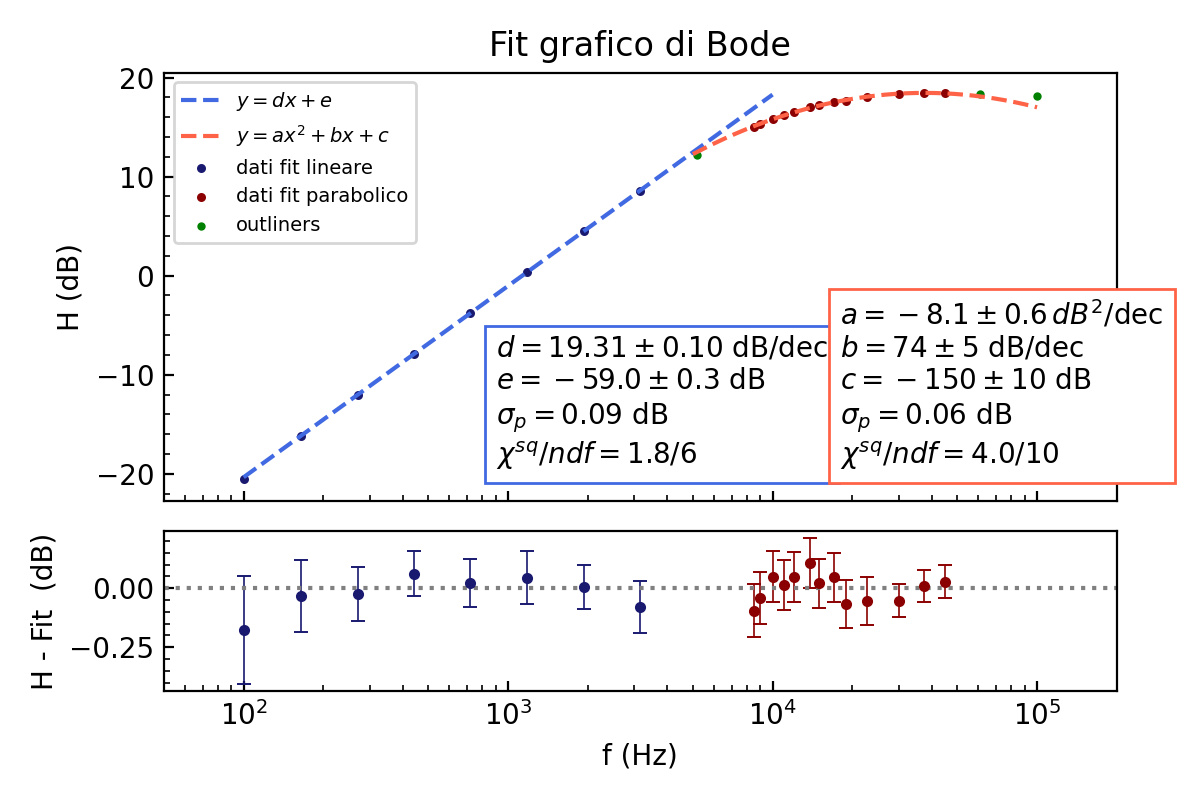
\includegraphics[width=0.8\textwidth]{images/fit_bode}
\caption{\footnotesize Nel grafico vengono riportati il fit lineare (in blu) e quello parabolico (in rosso). Si evidenziano inoltre gli outliners (in verde), non considerati durante i fit. In basso viene mostrato anche il grafico dei residui.}\label{fig:fit_bode}
\end{figure}
% -------------------------------------

\subsubsection{Stima frequenza di taglio in scala lineare}
\label{sec:stima-frequenza-di}

La strategia per stimare la frequenza di taglio del circuito dalla
funzione di trasferimento in scala lineare è la seguente:
si indivuidua un intorno della frequenza di taglio
sufficientemente stretto da evidenziare un andamento lineare dei dati in modo
da poter effettura un fit del tipo $y= fx + g$. In questo modo, è possibile
ricavare la frequenza di taglio dall'ascissa per cui l'intercetta vale
$H_{\text{max}}/\sqrt 2$
\begin{gather}
  \label{eq:ft_lin}
  f_{t} = \frac{H_{\text{max}} - \sqrt2 f}{\sqrt2 g}\\ 
  \sigma_{f_{t}} = f_t\sqrt{  \left( \frac{\sigma_{H_{\text{max}}}}{H_{\text{max}}-\sqrt2 f}\right)^2 + 
	  \left( \frac{\sigma_g}{\sqrt2 g}\right)^2 + 
	  \left( \frac{\sigma_f}{H_{\text{max}}-\sqrt2 f}\right)^2 + 
  2 \frac{\text{cov}(f,g)}{(H_\text{max}-\sqrt2 f)\sqrt 2 g}}
\end{gather}
dove l'errore sulla pendenza si ottiene sommando quadraticamente l'errore
del fit con i contributi di scala: poichè le misure nell'intervallo considerato
sono sono state prese con la stessa scala, gli errori sistematici
non alterano l'andamento dei residui e quindi nemmeno la bontà del fit.
Si decide quindi di considerare nell'interpolazione solamente gli errori di
lettura e correggere succesivamente l'incertezza sulla pendenza 
\begin{align}
	\sigma_{g}=\sqrt{\sigma_{g,\text{fit}}^2 + 2 g^2 \sigma_k^2 }
\end{align}
dove il fattore 2 deriva dalla presenza di due errori di scala, relativi ai due
segnali $V_{\text{in}}$ e $V_{\text{out}}$.
I risultati del fit sono riportati in Figura \ref{fig:fit_lin}. Si nota un'ottima compatibilità del chi quadro col suo valore atteso ($\lambda=0.7$), con una leggera sovrastima degli errori, evidenziata dalla deviazione standard a posteriori. Usando i risultati del fit nell'Equazione \ref{eq:ft_lin} e scegliendo $H_{\text{max}} = 8.36\pm 0.04$, cioè la stima ottenuta nella Sezione \ref{sec:grafico-di-bode} e convertita in scala lineare, segue che il nuovo valore della frequenza di taglio del circuito è $f_t=9.3 \pm 0.3 \,\si{k\Hz}$. Tale
stima è in ottimo accordo con le preivisioni teoriche calcolate nell'Equazione \ref{eq:f_teo} ($\lambda=0.8$).
%-------------------------------------
\begin{figure}[h]
\centering
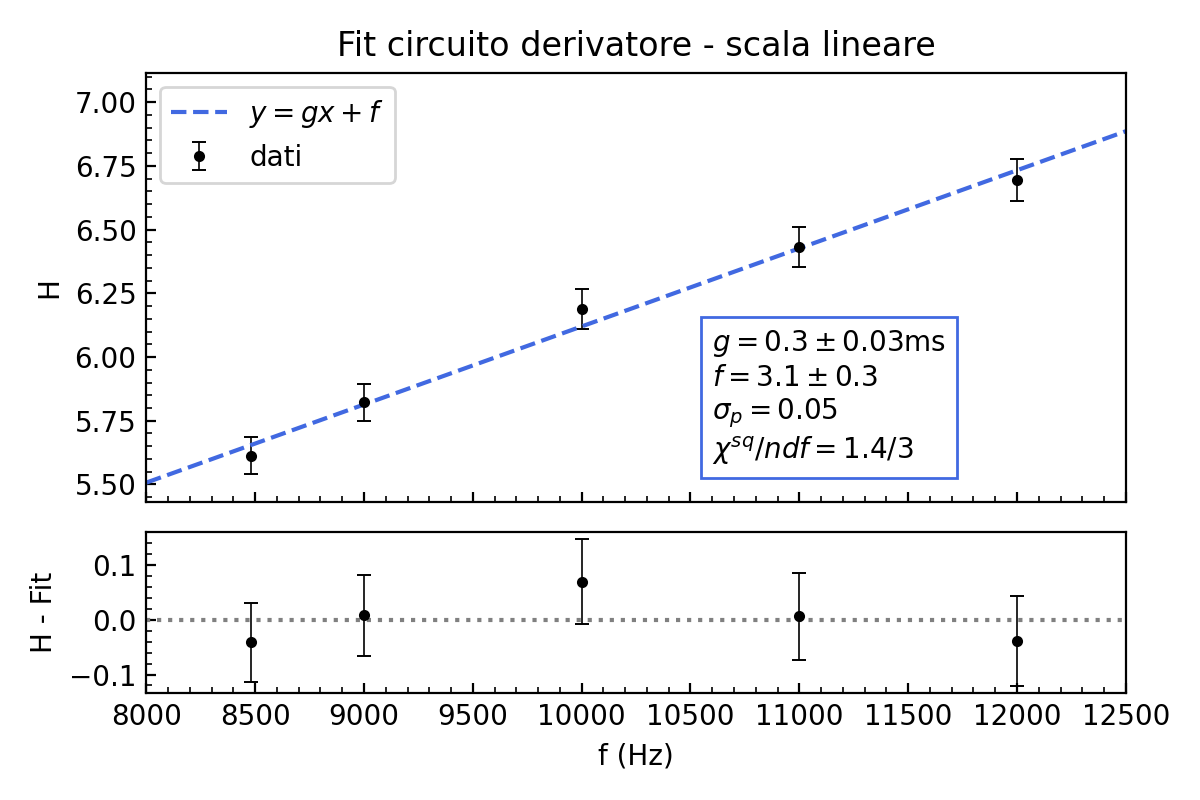
\includegraphics[width=0.8\textwidth]{images/fit_amp_lin}
\caption{\footnotesize Nella figura viene riportato il fit della funzione di trasferimento in scala
  lineare. In basso viene mostrato anche il grafico dei residui.}\label{fig:fit_lin}
\end{figure}
% -------------------------------------

\section{Circuito Sommatore}
\label{sec:circuito-sommatore}

In quest'ultima sezione ci si propone di verificare il comportamento di
sommatore invertente del circuito rappresentato in Figura \ref{fig:circ_sum}.

\subsection{Configurazione sperimentale}
\label{sec:conf-sper-1}

Il circuito utilizzato nella Sezione \ref{s:ampinv} viene modificato, sostituendo la resistenza di
feedback $R_{\text f}$ con la resistenza più simile a $R_{1}$ a
disposizione, $R_{2} = 8.06 \pm 0.04 \,k\Omega$ ($\lambda = 0.7 $). Inoltre, è stato aggiunto
un ingresso con la resistenza $R_{1\text b} = 8.08 \pm 0.04 \,k\Omega$, compatibile sia con $R_{1}$ ($\lambda  = 0.4$) che con $R_{2}$ ($\lambda = 0.4$).


%------------------------------------
\begin{wrapfigure}{r}{0.5\textwidth}
\centering
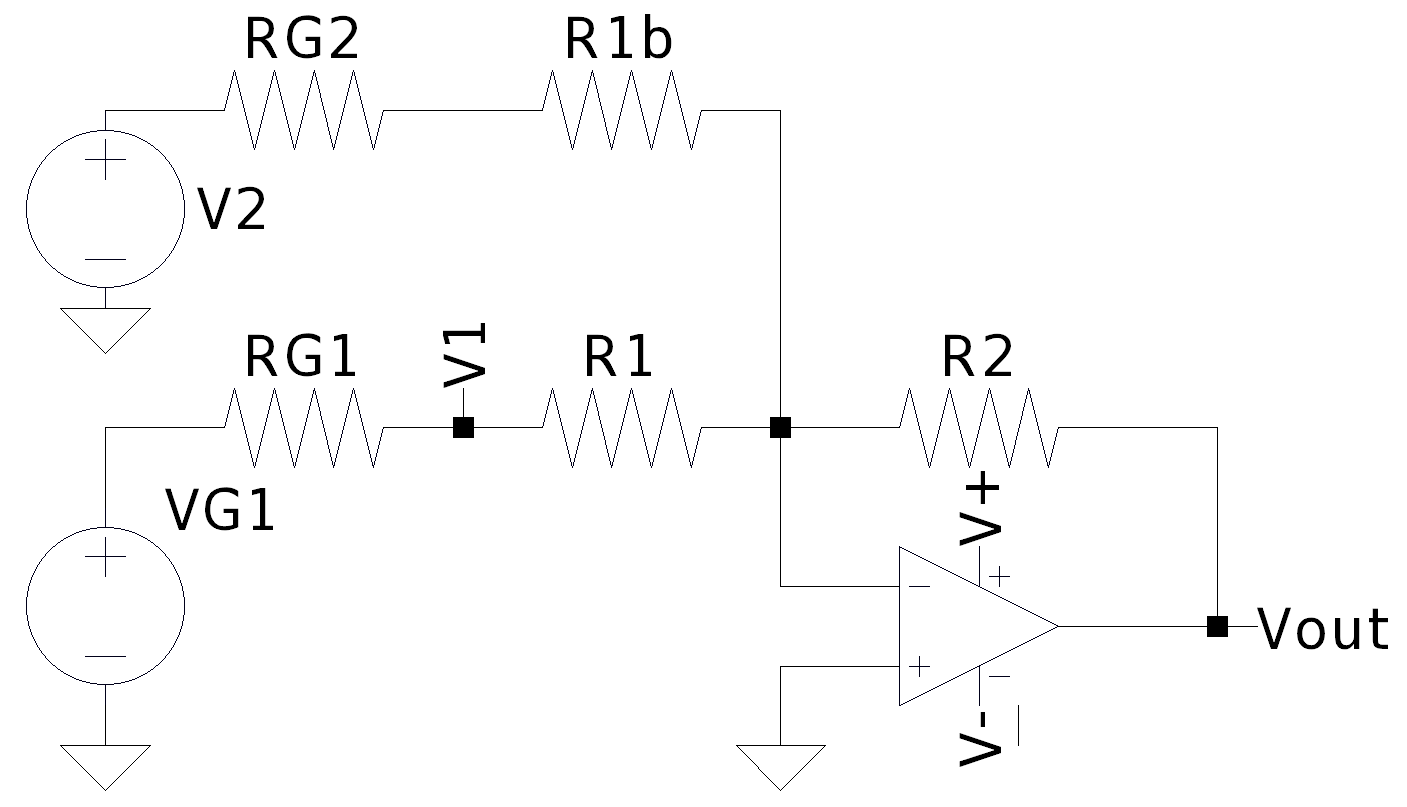
\includegraphics[width=0.5\textwidth]{images/circuit_sum}
\caption{\footnotesize Schema a variabili concentrate del circuito sommatore
  invertente utilizzato. Si noti la distinzione tra i punti $V_{G1}$ e $V_{1}$ dovuta dalla
  resistenza non trascurabile del generatore di funzioni. La resistenza $R_{G2}$ si assume
  invece trascurabile.}\label{fig:circ_sum}
\end{wrapfigure}
%------------------------------------


\noindent Sull'ingresso $V_{\text G1}$ viene applicata una tensione sinusoidale di ampiezza $2 \V$ e
frequenza $1\, \si{k\Hz}$, mentre l'ingresso $V_{2}$
viene collegato ad un generatore di tensione costante a $5\V$, incluso nella schedina
di alimentazione. Vengono quindi misurate con l'oscilloscopio le ampiezze dei segnali in ingresso
e in uscita. \\
Trattandosi di un sommatore pesato, ci si aspetta che valga la relazione
\begin{align}
  V_{\textrm{out}} = - \frac{R_{2}}{R_{1}} V_{1} - \frac{R_{2}}{R_{1\textrm b}} V_{2}
\end{align}
Data la compatibilità delle tre resistenze, l'equazione può essere
semplificata, e la risposta del circuito diventa semplicemente la somma
delle tensioni in ingresso, invertite di segno (si tratta comunque di un
amplificatore in configurazione invertente)
\begin{align}
  \label{eq:out_sum}
  V_{\textrm{out}} & = - (V_{1} + V_{2})
  &
   \sigma_{V_{\textrm{out}}}  &= \sqrt{ \sigma_{V_{1}}^{2} + \sigma_{V_{2}}^{2}}
\end{align}\label{eq:sum_th}
dove $\sigma_{V_{1}}$ e $\sigma_{V_{2}}$ rappresentano gli errori associati
alle misure dell'oscilloscopio, calcolati con l'Equazione \ref{e:err_misure}.
\subsection{Procedura di Acquisizione Dati}
\label{sec:acqu-delle-misure-1}

Inizialmente vengono sono utilizzate le due sonde collegate ai canali A e B
dell'oscilloscopio per registrare gli ingressi $V_{1}$ e $V_{2}$.
Si sceglie di acquisire per ogni segnale tre misure
coi cursori delle tensioni, in corrispondenza del massimo, del minimo
e del semiperiodo della sinusoidale del primo ingresso. Successivamente,
avendo a disposizione solo due canali nell'oscilloscopio, si sposta
la sonda B per registrare la tensione di uscita nei tre punti di
interesse.

\subsection{Dati e analisi}

Si vuole ora confrontare i dati acquisiti con le simulazioni
di LTspice. Si procede poi con un confronto tra le misure sperimentali e
il segnale in uscita previsto dall'Equazione \ref{eq:out_sum}.
In Tabella \ref{tab:mis_sum} sono riportate le misure acquisite.

%-----------------------------------
\begin{table}[h]
\centering
\setlength{\tabcolsep}{10pt}
\begin{tabular}{ |c|c|c|c|  }
  \hline
  \multicolumn{4}{|c|}{Misure significative sommatore invertente} \\
  \hline
  Descrizione & $V_{1}$  & $V_{2}$ & $V_{\text{out}}$\\
  \hline
  Massimo & $1.85 \pm 0.03 \V$ & $5.10 \pm 0.10 \V$ & $-6.94 \pm 0.13 \V$ \\
  Minimo & $-1.84 \pm 0.03 \V$ & $5.10 \pm 0.10 \V$ & $-3.25 \pm 0.07 \V$ \\
  Semiperiodo & $ 0.000 \pm 0.009 \V$ & $5.10 \pm 0.10 \V$ & $-5.07 \pm 0.10 \V$ \\
  \hline
\end{tabular}
\caption{\footnotesize Si mostrano in tabella i valori misurati con l'oscilloscopio e
  le relative incertezze. Si osservi che la sensiblità dell'oscilloscopio non è
  sufficiente a misurare nessuna cifra diversa da zero per la tensione $V_{1}$
  in corrispondenza del semiperiodo.
}\label{tab:mis_sum}
\end{table}
%-------------------------------------

\subsubsection{Simulazione del circuito}
\label{sec:simul-del-circ}

In Figura \ref{fig:sum_sim} vengono riportate due simulazioni del circuito ottenute con
LTspice, a cui vengono
sovraimposti i punti sperimentali. Tuttavia, poichè durante l'esperienza
si è preferito concentrarsi solo sui punti più significativi, non è stata
utilizzata la funzione per esporatre i dati direttamente dal Picoscope.
I valori mostrati in figura sono invece stati estrapolati da due screenshot
dell'oscilloscopio dal software WebPlotDigitizer. La prima simulazione (a sinistra
nella Figura \ref{fig:sum_sim}) viene effettuata usando come tensione del secondo ingresso il valore
nominale di $5 \V$. Si osserva però un leggero discostamento dai dati sperimentali
della tensione $V_{2}$, che presenta un offset verticale
$V_{\text{offset}}\approx 100\,\si{m\volt}$
che si riflette anche nell'andamento della tensione di uscita.
Si attribuisce questo effetto ad un background dovuto a delle interferenze
nella scheda di alimentazione. Si effettua quindi la seconda simulazione
(a destra) sostituendo al valore del secondo generatore la misura sperimentale
$V_{2}=5.10 \V$. Dalla Figura \ref{fig:sum_sim} si osserva chiaramente un migliore accordo
tra i dati sperimentali e la simulazione.
%------------------------------------
\begin{figure}[h]
\centering
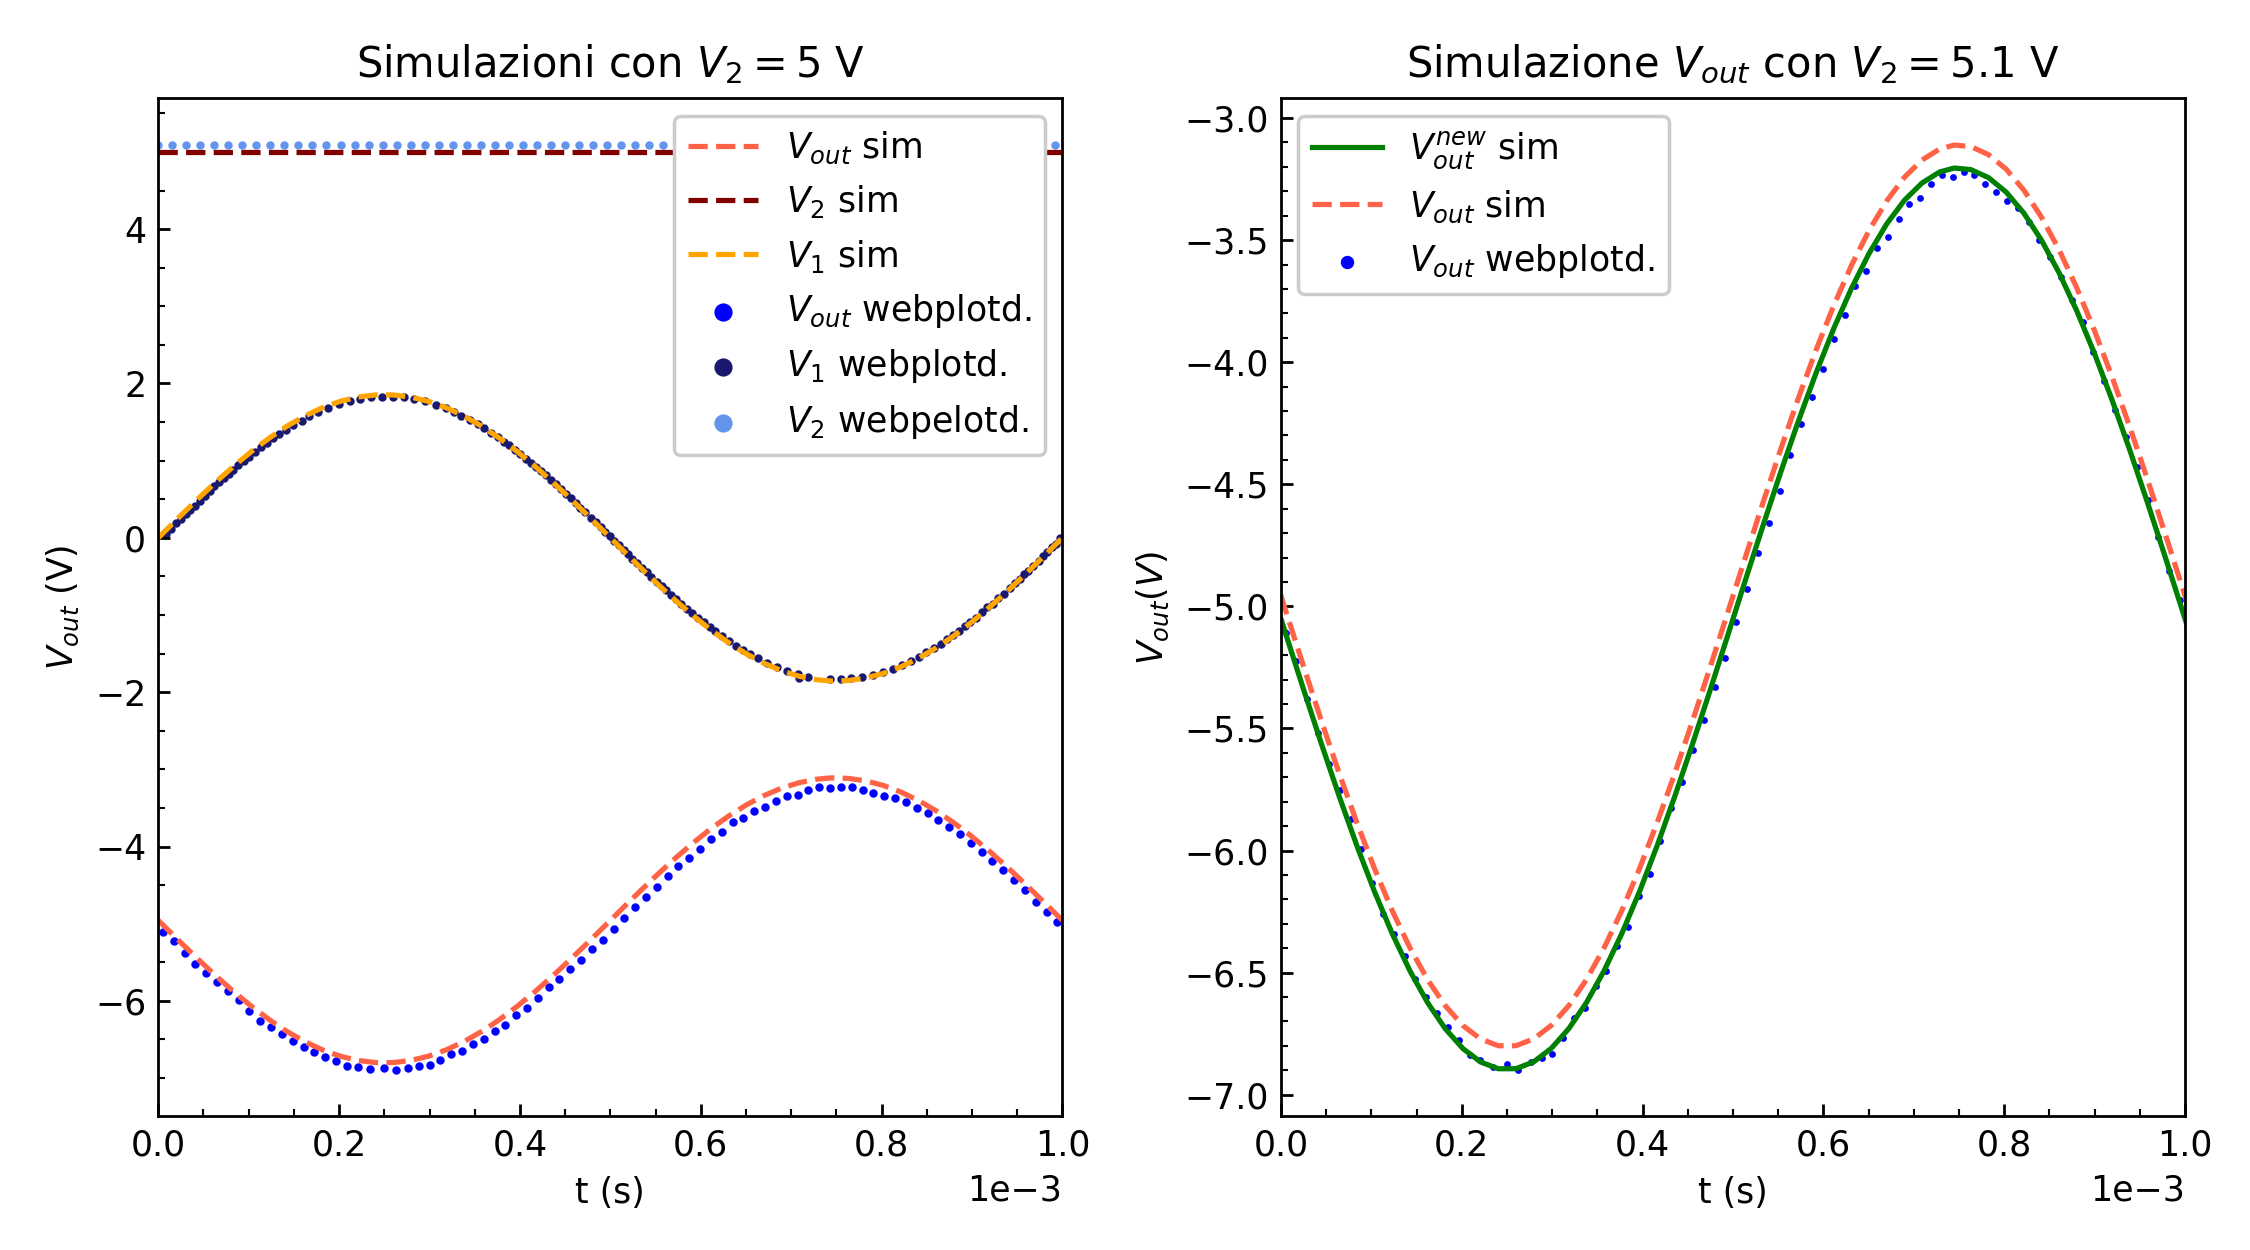
\includegraphics[width=1.0\textwidth]{images/sum_simulation}
\caption{\footnotesize Nel grafico a sinistra vengono riportate le simulazioni di LTspice (linee tratteggiate) e i dati estratti da WebPlotDigitizer, per tutti e tre i segnali. Nel
grafico a destra si mostra come la nuova simulazione ottenuta imponendo $V_{2}=5.1 \V$ descrive più fedelmente la tensione in uscita}\label{fig:sum_sim}
\end{figure}
%-------------------------------------

\subsubsection{Verifica del comportamento di sommatore}

Inserendo i dati della Tabella~\ref{tab:mis_sum} nell'equazione~\ref{eq:sum_th}, si prevedono i seguenti
valori di tensione in uscita:
\begin{align}
  \label{eq:11}
  V_{\text{out}}^{\text{max}} & = -6.94 \pm 0.11 \V
  &
    V_{\text{out}}^{\text{min}} & = -3.26 \pm 0.10 \V
  &
    V_{\text{out}}^{T/2}& = -5.10 \pm 0.18 \V
\end{align}
Nella tabella~\ref{tab:comp_sum} vengono confronati questi valori con quelli misurati: si osserva
un'ottima compatibilià per tutte e tre le misure, confermando quindi il comportamento
di circuito sommatore.
%-----------------------------------
\begin{table}
\centering
\setlength{\tabcolsep}{10pt}
\begin{tabular}{ |c|c|c|c|  }
  \hline
  \multicolumn{4}{|c|}{Compatibilità dati e previsioni} \\
  \hline
  Descizione & $V_{\text{out}}$ atteso  & $V_{\text{out}}$ misurato & $\lambda$\\
  \hline
  Massimo & $-6.94 \pm 0.11 \V$ & $-6.94 \pm 0.13 \V$ & $0.01$ \\
  Minimo & $-3.26 \pm 0.10 \V$ & $-3.25 \pm 0.07 \V$ & $0.1$ \\
  Semiperiodo & $ -5.10 \pm 0.10 \V$ & $-5.07 \pm 0.10 \V$ & $0.2$ \\
  \hline
\end{tabular}
\caption{\footnotesize Si mostrano in tabella i valori della tensione di uscita misurati con l'oscilloscopio e vengono confrontati con i valori previsti. Si mostra inoltre la compatibilità $\lambda$ tra le due stime.}\label{tab:comp_sum}
\end{table}
%-------------------------------------

\section{Conclusioni}
\label{sec:conclusioni}

Si riassume ora l'analisi effettuata nelle sezioni precedenti: si è cominciato verificando
la linearità dell'amplificatore operazionale dallo studio del fit in Figura~\ref{fig:lin_pp}, ottenuto
dai valori picco-picco delle tensioni misurate, così da eliminare la sistematica di offset
verticale osservata. La pendenza della retta interpolante ($G=8.56\pm 0.11$) corrisponde alla miglior
stima dell'amplificazione del circuito mostrato in Figura~\ref{fig:wrapfig}.
Nella Sezione~\ref{sec:circuito-derivatore} si è poi verificato il comportamento da derivatore
del circuito rappresentato in Figura~\ref{fig:circ_bode} e si è studiata la sua risposta in
frequenza con l'obietivo di ottenere una stima della frequenza
di taglio: dall'analisi del grafico di Bode in Figura~\ref{fig:fit_bode} si è ottenuta una
prima stima $f_{t}=10.21\pm 0.14 \,\si{k\Hz}$, scarsamente compatibile con l'aspettativa teorica a causa
delle sistematiche evidenziate dal grafico dei residui.
Si è poi sposta l'attenzione sull'analisi in scala lineare, e dall'interpolazione mostata in Figura~\ref{fig:fit_lin} si è ottenuto $f_{t}=9.3\pm 0.3 \,\si{k\Hz}$, in ottima compatibilità con le aspettative teoriche.
Si assume quindi questa come miglior stima della freqeunza di taglio del circuito.
Infine, nella Sezione~\ref{sec:circuito-sommatore} si è verificato il comportamento di sommatore invertente del circuito rappresentato in Figura~\ref{fig:circ_sum}: inizialmente vengono confrontati i dati con le simulazioni ottenute
con LTspice, da cui si evidenzia un segnale di fondo di $\approx 100 \,\si{m\volt}$ dovuto a
interferenza nella scheda di alimentazione. Sono state poi confrontatoi i dati sperimentali con le aspettative teoriche in corrispondenza del massimo, del minimo
e del semiperiodo del segnale del generatore di funzioni. In tutti e tre i casi si è riscontra
 un'ottima compatibilità con le previsioni, come si evince dalla Tabella~\ref{tab:comp_sum}.
\end{document}
